% Para utilizar este template siga o tutorial disponível em http://www.biblioteca.ufc.br/wp-content/uploads/2015/09/tutorial-sharelatex.pdf

%%%%%%%%%%%%%%%%%%%%%%%%%%%%%%%%%%%%%%%%%%%%%%%%%%%%%%%
%% Você deve criar uma conta no Overleaf. Depois,    %%
%% vá nas opções no canto esquerdo superior da tela  %%
%% e clique em "Copiar Projeto". Dê um novo nome pa- %%
%% ra o projeto.                                     %%
%%                                                   %%
%% Os principais desenvolvedores deste template são: %%
%%                                                   %%
%%            Ednardo Moreira Rodrigues              %%
%%       (Doutor em Engenharia Elétrica - UFC)       %%
%%                      &                            %%
%%            Alan Batista de Oliveira               %%
%%           (Engenheiro Eletricista - UFC)          %%
%%                                                   %%
%% Consultoria Bibliotecária                         %%
%%                                                   %%
%%  Versão 2016 - ShareLaTeX:                        %%
%%                                                   %%
%% - Francisco Edvander Pires Santos;                %%
%% - Juliana Soares Lima;                            %%
%% - Izabel Lima dos Santos;                         %%
%% - Kalline Yasmin Soares Feitosa;                  %%
%% - Eliene Maria Vieira de Moura.                   %%
%%
%%  Versão 2019 - Overleaf:
%%
%%  Biblioteca de Ciências Humanas:
%% - Francisco Edvander Pires Santos;                %%
%% - Juliana Soares Lima;                            %%
%% - Eliene Maria Vieira de Moura;                   %%
%% - Edmundo Moreira de Sousa Filho.                 %%
%%                                                   %%
%% Biblioteca da FEAAC:                              %%
%% - Izabel Lima dos Santos;                         %%
%% - Kalline Yasmin Soares Feitosa;                  %%
%% - Kleber Lima dos Santos.                         %%
%%                                                   %%
%%  Biblioteca do Curso de Física:                   %%
%% - Aline Rodrigues de Lima Mendes;                 %%
%% - Maria de Jesus Silva dos Santos.                %%
%%                                                   %%
%%  Biblioteca Central do Campus do Pici:            %%
%% - Raquel da Silva Nascimento.                     %%
%%                                                   %%
%% Colaboradores                                     %%
%%                                                   %%
%% -Andrei Bosco Bezerra Torres                      %%
%% (Professor - Sistemas e Mídias Digitais -         %%
%% Instituto Universidade Virtual - UFC)             %%
%% Tiago ALves Lima                                  %%
%% (Aluno de Mestrado em Eng. Elétrica)              %%
%%                                                   %%
%% Grande parte do trabalho foi adaptado do template %%
%% da UECE elaborado por:                            %%
%% Thiago Nascimento  (UECE)                         %%
%% Project available on:                             %%
%% https://github.com/thiagodnf/uecetex2             %%
%%                                                   %%
%% "Dúvidas, esclarecimentos ou sugestões podem ser  %%
%% enviadas para o seguinte e-mail:                  %%
%%                                                   %%
%%             atendimentobch@ufc.br                 %%
%%                                                   %%
%% As últimas atualizações estão descritas no inicio %%
%% do arquivo "README.md".                           %%
%%                                                   %%
%%%%%%%%%%%%%%%%%%%%%%%%%%%%%%%%%%%%%%%%%%%%%%%%%%%%%%%

\documentclass[
    a4paper,          % Tamanho da folha A4
    12pt,             % Tamanho da fonte 12pt
    chapter=TITLE,    % Todos os capitulos devem ter caixa alta
    section=Title,    % Todas as secoes devem ter caixa alta somente na primeira letra
    subsection=Title, % Todas as subsecoes devem ter caixa alta somente na primeira letra
    oneside,          % Usada para impressao em apenas uma face do papel
    english,          % Hifenizacoes em ingles
    spanish,          % Hifenizacoes em espanhol
    brazil,           % Ultimo idioma eh o idioma padrao do documento
    fleqn             % Comente esta linha se quiser centralizar as equacoes. Comente também a linha 65 abaixo
]{abntex2}

% Para utilizar este template siga o tutorial disponível em http://www.biblioteca.ufc.br/wp-content/uploads/2015/09/tutorial-sharelatex.pdf

%%%%%%%%%%%%%%%%%%%%%%%%%%%%%%%%%%%%%%%%%%%%%%%%%%%%%%%
%% Você deve criar uma conta no Overleaf. Depois,    %%
%% vá nas opções no canto esquerdo superior da tela  %%
%% e clique em "Copiar Projeto". Dê um novo nome pa- %%
%% ra o projeto.                                     %%
%%                                                   %%
%% Os principais desenvolvedores deste template são: %%
%%                                                   %%
%%            Ednardo Moreira Rodrigues              %%
%%       (Doutor em Engenharia Elétrica - UFC)       %%
%%                      &                            %%
%%            Alan Batista de Oliveira               %%
%%           (Engenheiro Eletricista - UFC)          %%
%%                                                   %%
%% Revisão:                                          %%
%%                                                   %%
%% - Francisco Edvander Pires Santos;                %%
%% - Juliana Soares Lima;                            %%
%% - Izabel Lima dos Santos;                         %%
%% - Kalline Yasmin Soares Feitosa.                  %%
%% - Eliene Maria Vieira de Moura;                   %%
%%                                                   %%
%% Colaboradores                                     %%
%%                                                   %%
%% -Andrei Bosco Bezerra Torres                      %%
%% (Professor - Sistemas e Mídias Digitais -         %%
%% Instituto Universidade Virtual - UFC)             %%
%% Tiago ALves Lima                                  %%
%% (Aluno de Mestrado em Eng. Elétrica)              %%
%%                                                   %%
%% Grande parte do trabalho foi adaptado do template %%
%% da UECE elaborado por:                            %%
%% Thiago Nascimento  (UECE)                         %%
%% Project available on:                             %%
%% https://github.com/thiagodnf/uecetex2             %%
%%                                                   %%
%% "Dúvidas, esclarecimentos ou sugestões podem ser  %%
%% enviadas para o seguinte e-mail:                  %%
%%                                                   %%
%%             atendimentobch@ufc.br                 %%
%%                                                   %%
%% As últimas atualizações estão descritas no inicio %%
%% do arquivo "README.md".                           %%
%%                                                   %%
%%%%%%%%%%%%%%%%%%%%%%%%%%%%%%%%%%%%%%%%%%%%%%%%%%%%%%%

% Importações de pacotes
\usepackage[utf8]{inputenc}                         % Acentuação direta
\usepackage[T1]{fontenc}                            % Codificação da fonte em 8 bits
\usepackage{graphicx}                               % Inserir figuras
\usepackage{amsfonts, amssymb, amsmath}             % Fonte e símbolos matemáticos
\usepackage{booktabs}                               % Comandos para tabelas
\usepackage{verbatim}                               % Texto é interpretado como escrito no documento
\usepackage{multirow, array}                        % Múltiplas linhas e colunas em tabelas
\usepackage{indentfirst}                            % Endenta o primeiro parágrafo de cada seção.
\usepackage{listings}                               % Utilizar codigo fonte no documento
\usepackage[table,xcdraw]{xcolor}
\usepackage{xcolor}
\usepackage{microtype}                              % Para melhorias de justificação?
\usepackage[portuguese,ruled,lined]{algorithm2e}    % Escrever algoritmos
\usepackage{algorithmic}                            % Criar Algoritmos
%\usepackage{float}                                 % Utilizado para criação de floats
\usepackage{amsgen}
\usepackage{lipsum}                                 % Usar a simulação de texto Lorem Ipsum
%\usepackage{titlesec}                              % Permite alterar os títulos do documento
\usepackage{tocloft}                                % Permite alterar a formatação do Sumário
\usepackage{etoolbox}                               % Usado para alterar a fonte da Section no Sumário
\usepackage[nogroupskip,nonumberlist]{glossaries}   % Permite fazer o glossario

\usepackage[font=singlespacing,format=plain,justification=justified,skip=0pt,singlelinecheck = false]{caption}            % Altera o comportamento da tag caption

\usepackage[alf, abnt-emphasize=bf, recuo=0cm, abnt-etal-cite=2, abnt-etal-list=0, abnt-etal-text=it]{abntex2cite}  % Citações padrão ABNT
%\usepackage[bottom]{footmisc}                      % Mantém as notas de rodapé sempre na mesma posição
%\usepackage{times}                                 % Usa a fonte Times
%%%%%%%%%%%%%%%%%%% AVISO %%%%%%%%%%%%%%%%%%%%%%%%%%%%%%%%%%%%%%%%
%descomente as duas linhas abaixo para alterar o texto de Times New Roman para Arial:

%\usepackage{helvet}
%\renewcommand{\familydefault}{\sfdefault}  % Usa a fonte Arial
%%%%%%%%%%%%%%%%%%%%%%%%%%%%%%%%%%%%%%%%%%%%%%%%%%%%%%%%%%%%%%%%%%

\usepackage{mathptmx}         % Usa a fonte Times New Roman			%\usepackage{lmodern}         % Usa a fonte Latin Modern
%\usepackage{subfig}          % Posicionamento de figuras
%\usepackage{scalefnt}        % Permite redimensionar tamanho da fonte
%\usepackage{color, colortbl} % Comandos de cores
%\usepackage{lscape}          % Permite páginas em modo "paisagem"
%\usepackage{ae, aecompl}     % Fontes de alta qualidade
%\usepackage{picinpar}        % Dispor imagens em parágrafos
%\usepackage{latexsym}        % Símbolos matemáticos
%\usepackage{upgreek}         % Fonte letras gregas
\usepackage{appendix}         % Gerar o apendice no final do documento
\usepackage{paracol}          % Criar paragrafos sem identacao
\usepackage{lib/ufctex}	      % Biblioteca com as normas da UFC para trabalhos academicos
\usepackage{pdfpages}         % Incluir pdf no documento
\usepackage{amsmath}          % Usar equacoes matematicas


\makeglossaries% Organiza e gera a lista de abreviaturas, simbolos e glossario
\makeindex     % Gera o Indice do documento


\setlength{\mathindent}{0pt} %Complementa o alinhamento de equações para totalmente a esquerda.

%%%%%%%%%%%%%%%%%%%%%%%%%%%%%%%%%%%%%%%%%%%%%%%%%%%%%
%%                     ATENCAO                     %%
%%%%%%%%%%%%%%%%%%%%%%%%%%%%%%%%%%%%%%%%%%%%%%%%%%%%%
%  Qual e o nivel do trabalho academico que voce esta
% escrevendo? Retire o simbolo "%" apenas de um dos
% quatro topicos abaixo refente ao nível do seu traba
% -lho.

\trabalhoacademico{tccgraduacao}
%\trabalhoacademico{tccespecializacao}
%\trabalhoacademico{dissertacao}
%\trabalhoacademico{tese}

%%%%%%%%%%%%%%%%%%%%%%%%%%%%%%%%%%%%%%%%%%%%%%%%%%%%%

% Define se o trabalho e uma qualificacao
% Coloque 'nao' para versao final do trabalho

\ehqualificacao{nao}

% Remove as bordas vermelhas e verdes do PDF gerado
% Coloque 'sim' pare remover

\removerbordasdohyperlink{sim}

% Adiciona a cor Azul a todos os hyperlinks

\cordohyperlink{nao}

%%%%%%%%%%%%%%%%%%%%%%%%%%%%%%%%%%%%%%%%%%%%%%%%%%%%%
%%         Informacao sobre a instituicao          %%
%%%%%%%%%%%%%%%%%%%%%%%%%%%%%%%%%%%%%%%%%%%%%%%%%%%%%

\ies{Universidade Federal do Ceará}
\iessigla{UFC}
\centro{Campus de Sobral}
\departamento{Departamento de Computação}

%%%%%%%%%%%%%%%%%%%%%%%%%%%%%%%%%%%%%%%%%%%%%%%%%%%%%
%%        Informacao para TCC de Graduacao         %%
%%%%%%%%%%%%%%%%%%%%%%%%%%%%%%%%%%%%%%%%%%%%%%%%%%%%%

\graduacaoem{Engenharia da Computação}
\habilitacao{bacharel} % Ou licenciado(a)

% AVISO: Caso necessario alterar o texto de apresenta-
% cao da Especializacao, ir a pasta "lib", arquivo
% "ufctex.sty" na linha 502.


%%%%%%%%%%%%%%%%%%%%%%%%%%%%%%%%%%%%%%%%%%%%%%%%%%%%%
%%     Informacao para TCC de Especializacao       %%
%%%%%%%%%%%%%%%%%%%%%%%%%%%%%%%%%%%%%%%%%%%%%%%%%%%%%

\especializacaoem{Yyyyyyyyy}

% AVISO: Caso necessario alterar o texto de apresenta-
% cao da Especializacao, ir a pasta "lib", arquivo
% "ufctex.sty" na linha 507.

%%%%%%%%%%%%%%%%%%%%%%%%%%%%%%%%%%%%%%%%%%%%%%%%%%%%%
%%         Informacao para Dissertacao             %%
%%%%%%%%%%%%%%%%%%%%%%%%%%%%%%%%%%%%%%%%%%%%%%%%%%%%%

\programamestrado{Programa de Pós-Graduação em Xxxxxxx}
\nomedomestrado{Mestrado Acadêmico em Xxxxxxx}
\mestreem{Engenharia Xxxxxx}
\areadeconcentracaomestrado{Engenharia Xxxxxx}

% AVISO: Caso necessario alterar o texto de apresenta-
% cao da dissertacao, ir a pasta "lib", arquivo
% "ufctex.sty" na linha 511.

%%%%%%%%%%%%%%%%%%%%%%%%%%%%%%%%%%%%%%%%%%%%%%%%%%%%%
%%               Informação para Tese              %%
%%%%%%%%%%%%%%%%%%%%%%%%%%%%%%%%%%%%%%%%%%%%%%%%%%%%%

\programadoutorado{Programa de Pós-Graduação em Xxxxxx}
\nomedodoutorado{Doutorado em Xxxxxxx}
\doutorem{Engenharia Xxxxxx}
\areadeconcentracaodoutorado{Engenharia Xxxxxxx}

% AVISO: Caso necessario alterar o texto de apresenta-
% cao da tese, ir a pasta "lib", arquivo "ufctex.sty"
% na linha 515.

%%%%%%%%%%%%%%%%%%%%%%%%%%%%%%%%%%%%%%%%%%%%%%%%%%%%%
%%      Informacoes relacionadas ao trabalho       %%
%%%%%%%%%%%%%%%%%%%%%%%%%%%%%%%%%%%%%%%%%%%%%%%%%%%%%

\autor{Manoel Vilela Machado Neto}
\titulo{Segmentação Semi-Supervisionada de Imagens através de
Dinâmicas Coletivas em Redes Complexas}
\data{2022}
\local{Sobral}

% Exemplo: \dataaprovacao{01 de Janeiro de 2012}
\dataaprovacao{}

%%%%%%%%%%%%%%%%%%%%%%%%%%%%%%%%%%%%%%%%%%%%%%%%%%%%%
%%           Informação sobre o Orientador         %%
%%%%%%%%%%%%%%%%%%%%%%%%%%%%%%%%%%%%%%%%%%%%%%%%%%%%%

\orientador{Prof.\ Dr.\ Jarbas Joaci de Mesquita Sá Junior}
\orientadories{Universidade Federal do Ceará (UFC)}
\orientadorcentro{Centro de Ciências e Tecnologia (CCT)}
\orientadorfeminino{nao} % Coloque 'sim' se for do sexo feminino

%%%%%%%%%%%%%%%%%%%%%%%%%%%%%%%%%%%%%%%%%%%%%%%%%%%%%
%%          Informação sobre o Coorientador        %%
%%%%%%%%%%%%%%%%%%%%%%%%%%%%%%%%%%%%%%%%%%%%%%%%%%%%%

% Deixe o nome do coorientador em branco para remover do documento

% \coorientador{Prof. Dr. Filipe A. N. Verri}
% \coorientadories{Instituto Tecnológico da Aeronaútica (ITA)}
% \coorientadorcentro{Divisão de Ciência da Computação (IEC)}
% \coorientadorfeminino{nao} % Coloque 'sim' se for do sexo feminino

%%%%%%%%%%%%%%%%%%%%%%%%%%%%%%%%%%%%%%%%%%%%%%%%%%%%%
%%              Informação sobre a banca           %%
%%%%%%%%%%%%%%%%%%%%%%%%%%%%%%%%%%%%%%%%%%%%%%%%%%%%%

% Atenção! Deixe em branco o nome do membro da banca para remover da folha de aprovacao

% Exemplo de uso:
% \membrodabancadois{Prof. Dr. Fulano de Tal}
% \membrodabancadoisies{Universidade Federal do Ceará - UFC}


\membrodabancadois{Prof.\ Dr.\ Xxxxxxx Xxxxxx Xxxxxxx}
\membrodabancadoiscentro{Centro de Ciências e Tecnologia (CCT)}
\membrodabancadoisies{Universidade Federal do Ceará (UFC)}
\membrodabancatres{Prof.\ Dr.\ Xxxxxxx Xxxxxx Xxxxxxx}
\membrodabancatrescentro{Centro de Ciências e Tecnologia (CCT)}
\membrodabancatresies{Universidade Federal do Ceará (UFC)}
% \membrodabancaquatro{Prof. Dr. Xxxxxxx Xxxxxx Xxxxxxx}
% \membrodabancaquatrocentro{Centro de Ciências e Tecnologia (CCT)}
% \membrodabancaquatroies{Universidade do Membro da Banca Quatro (SIGLA)}
% \membrodabancacinco{Prof. Dr. Xxxxxxx Xxxxxx Xxxxxxx}
% \membrodabancacincocentro{Teste}
% \membrodabancacincoies{Universidade do Membro da Banca Cinco (SIGLA)}
% \membrodabancaseis{Prof. Dr. Xxxxxxx Xxxxxx Xxxxxxx}
% \membrodabancaseiscentro{}
% \membrodabancaseisies{Universidade do Membro da Banca Seis (SIGLA)}
%
\begin{document}

    % Elementos pré-textuais
    \imprimircapa{}
    %\imprimirfolhaderosto{}
	%\imprimirfichacatalografica{1-pre-textuais/ficha-catalografica}
	%\imprimirerrata{elementos-pre-textuais/errata}
	\imprimirfolhadeaprovacao{}
	\imprimirdedicatoria{1-pre-textuais/dedicatoria}
	\imprimiragradecimentos{1-pre-textuais/agradecimentos}
	\imprimirepigrafe{1-pre-textuais/epigrafe}
	\imprimirresumo{1-pre-textuais/resumo}
	\imprimirabstract{1-pre-textuais/abstract}
    % Se você comentar esta linha o título da lista fica: LISTA DE ILUSTRAÇÕES
	\renewcommand*\listfigurename{Lista de Figuras}
	\imprimirlistadeilustracoes{}
	%\imprimirlistadetabelas
	%\imprimirlistadequadros
	%\imprimirlistadealgoritmos
	%\imprimirlistadecodigosfonte
	\imprimirlistadeabreviaturasesiglas{}
	%\imprimirlistadesimbolos{1-pre-textuais/lista-de-simbolos}
	\imprimirsumario{}

	\setcounter{table}{0}% Deixe este comando antes da primeira tabela.

	%Elementos textuais
	\textual{}
	\chapter{INTRODUÇÃO}\label{cap:introducao}

Sistemas de segmentação de imagens têm se tornado populares em
variadas aplicações, como, por exemplo, a área de edição de imagem,
diagnósticos médicos e parte da visão computacional necessária pra
reconhecimento de objetos. Entre esses motivos e outros, essa área tem
uma relevância científica alta considerando a situação social,
tecnológica e econômica que é vivida no século XXI.\@

A segmentação de uma imagem pode ser feita manualmente por um anotador
humano marcando as linhas delineadoras de um objeto. Por outro lado,
são conhecido algoritmos variados para segmentação de imagens baseados
em aprendizagem de máquina, que através de exemplos de segmentação
fornecidos para treinamento é possível inferir a segmentação de novas imagens.

Na Figura~\ref{fig:image-segmentation-types} é apresentado um quadro
comparativo de operações em uma imagem com balões, incluindo os tipos
de segmentação de imagens conhecidos: semântica e instância. Na
segmentação semântica o objetivo é segmentar apenas os mesmos tipos de
objetos como o mesmo rótulo, na segmentação por instância, cada balão
é visto como a mesma classe de balão mas com rótulos associados diferentes.

\begin{figure}[h!]
        \captionsetup{width=16cm}
		\Caption{\label{fig:image-segmentation-types}
Comparação de tipos de segmentação de imagem: por semântica e instância
}
		\centering
		\UFCfig{}{\fbox{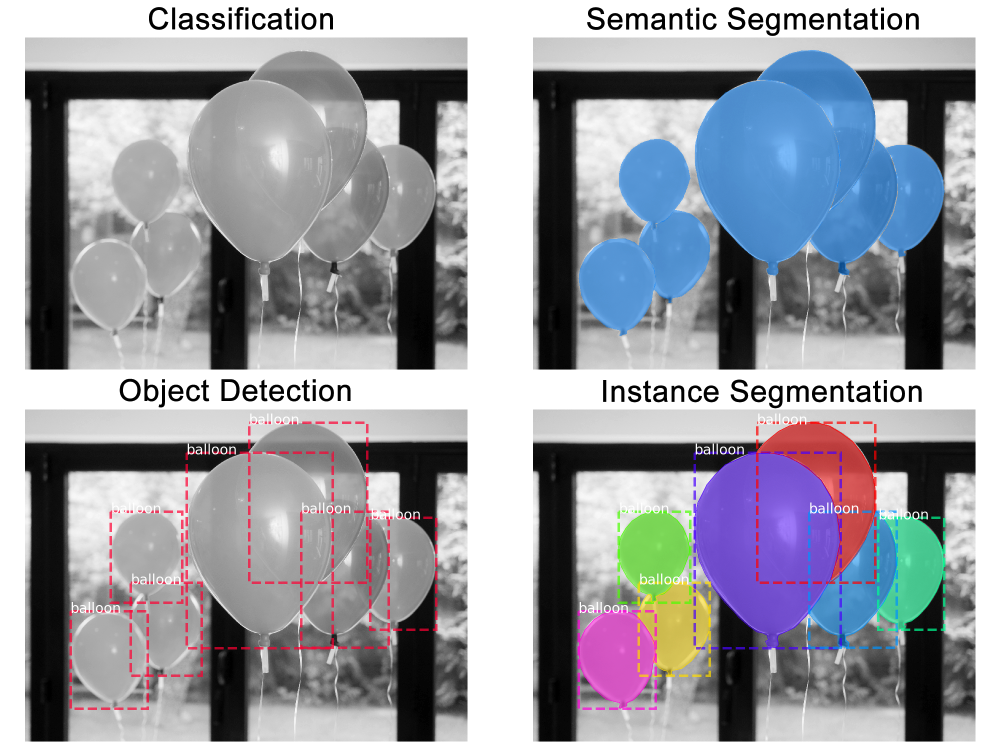
\includegraphics[width=16cm]{figuras/image-segmentation-types}}}{\Fonte{\citeonline{MediumInstanceSegmentation2019}}}
\end{figure}


Entre os tipos de aprendizagem de máquina, para segmentação de imagens
semântica é selecionada neste trabalho especificamente a aprendizagem
semi-supervisionada transdutiva\footnote{mais informações na
seção~\ref{sec:teorica-aprendizado-semi-supervisionado}}. A
aprendizagem semi-supervisionada é uma categoria que realiza o
aprendizado com poucas rotulações e maior parte dos dados não são
rotulados. Outras categorias de aprendizado de máquina como
supervisionada possui no treinamento uma base totalmente rotulada
enquanto a aprendizagem não-supervisionada não possui rótulo algum
(exemplo: K-means). Ao considerar a dificuldade de conseguir dados
rotulados por humanos em ambientes de uso por especialistas, como imagens
médicas e ferramentas de edição de imagem, a abordagem
semi-supervisionada se demonstra interessante por precisar de poucos
dados rotulados, mas ainda existir uma anotação com viés do
especialista interessado (médico, editor).


Os três principais algoritmos clássicos de segmentação de imagem podem
ser citados: \textit{Region-Based Segmentation}; \textit{Edge Detection
  Segmentation}; \textit{Segmentation based on Clustering}
~\cite{ImageSegmentationTechniques1985}. Cada uma dessas técnicas
possui limitações conhecidas, e entre elas é possível mencionar: haver
muitos objetos na imagem pode dificultar a segmentação; tempo
computacional elevado; sensibilidade ao contraste em escala cinza.

Um cenário especial de segmentação semântica abordado neste trabalho
para aplicação de um esquema de aprendizagem semi-supervisionada é o
problema de segmentação interativa\footnote{conceito explicado em
detalhes na seção ~\ref{sec:segmentacao-interativa}}, onde o objetivo
é uma segmentação binária que busca segmentar um objeto alvo em
relação ao plano de fundo.

Considerando tal situação-problema, este trabalho propõe a construção
de uma técnica de segmentação de imagem semi-supervisionada voltada
para segmentação interativa utilizando redes complexas e dinâmicas
coletivas de tal maneira que possa se equiparar as melhores técnicas
atuais de segmentação interativa baseado em grafos.

\section{Trabalhos relacionados}\label{cap:trabalhos-relacionados}

Técnicas de segmentação de imagens com o paradigma semi-supervisionado
estão em foco atualmente no campo médico, como pode ser visto em
~\cite{LuoSemiSupervised2021}. Nesse artigo, uma das grandes
motivações de os autores utilizarem uma técnica semi-supervisionada
está relacionado com a dificuldade de possuir dados anotados de dados
em um domínio de dados, como imagens hospitalares.

Em relação ao tópico de redes complexas e dinâmicas coletivas, é
possível mencionar o trabalho feito com o algoritmo \gls{LCU}
~\cite{VerriNetworkUnfoldingMap2018} no qual os principais conceitos
sobre resolução de problemas de aprendizagem de máquina
semi-supervisionada são explorados em detalhes como uma dinâmica de
competição de partículas na relação vértice-arestas de um grafo
não-direcionado. Este método de aprendizagem é transdutivo, portanto,
difere dos métodos indutivos que estimam uma função de inferência no
treinamento, como é o caso de Redes Neurais. Além disso, esse
algoritmo tem complexidade computacional linear em relação à
quantidade de classes, arestas e vértices.

Para ilustrar uma possível ideia de segmentação de imagens, ao
considerar um algoritmo que faça uma transformação do domínio de
imagem para um grafo, é possível estabelecer uma relação na qual os
vértices representam parte da imagem como um \textit{superpixel}
~\cite{SuperpixelSurvey2020}, ou seja, um grupo de subpixels da
imagem. Na Figura~\ref{fig:segmentation-superpixel} é apresentado um
exemplo de segmentação usando superpixels. Algoritmos de superpixel
são não-supervisionados em geral, portanto possuem suas limitações
quanto ao resultado esperado pelo usuário \textendash\hfill logo
difícil de ser aceito em aplicações médicas nas quais a opinião do
especialista é de alta relevância para o resultado final.

\begin{figure}[!h]
        \captionsetup{width=9cm}
		\Caption{\label{fig:segmentation-superpixel}
          Segmentação superpixel}
		\centering
		\UFCfig{}{
			\fbox{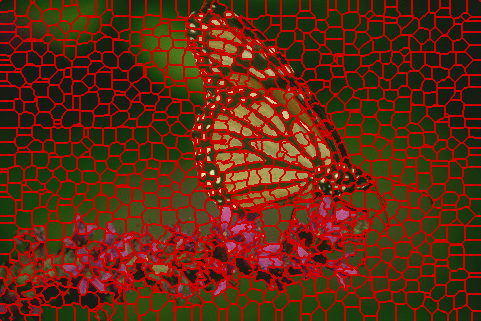
\includegraphics[width=9cm]{figuras/example-superpixel-segmentation}}
		}{
			\Fonte{\cite{SuperPixelBenchmark2017}}
		}
\end{figure}



Seguindo essa perspectiva, ao utilizar um algoritmo de extração de
\textit{features} de imagens sobre o superpixel, tem-se que o vértice
do grafo é neste momento um vetor de características. O sistema de
competição proposto no artigo \textit{Network Unfolding Map By
Vertex-Edge Dynamics Modeling} pode otimizar o pertencimento de
classes (segmentos, nesse caso) baseado na topologia de sua vizinhança
e na relação aos vértices conectados. A métrica de similaridade
(por exemplo, distância euclidiana, cosseno, etc.) pode ser
ajustada de acordo com o problema.

Ao considerar o problema como semi-supervisionado, a pista de ter
alguns dos superpixels anotados adicionaria um \textit{bias}
parametrizado pelo conhecimento do especialista em uso da ferramenta,
como um editor ou um médico. A otimização do pertencimento das classes
então seria acionada pela dinâmica coletiva selecionada em questão,
que, por acaso, poderia ser o algoritmo \gls{LCU} mencionado anteriormente.

Por outro lado, ainda há muitas melhorias a serem feitas nessas técnicas, como,
por exemplo: analisar as condições de convergência do algoritmo. Isso
pode ser um dos resultados deste trabalho, demandando uma análise
matemática com auxílio de experimentos.

É importante mencionar que já foi demonstrado em outras situações,
como em~\cite{JarbasComplexNetworks2020}, que o uso de redes complexas
em fusão com redes neurais aleatórias pode gerar um discriminante de
textura da imagem de alta relevância como extrator de
características. Neste caso, é possível se apoiar nesse resultado como
uma evidência de que a investigação de novas técnicas considerando a
topologia da imagem através de redes complexas é uma oportunidade de
pesquisa.


\subsection{GrabCut: Interactive Foreground Extraction Using Iterated
  Graph Cuts}\label{sec:grabcut}

Neste trabalho, um dos pioneiros em segmentação interativa, os
autores~\cite{rother2004grabcut} desenvolveram uma técnica para segmentação interativa
chamada GrabCut baseado em um mapeamento da imagem como um grafo e
então um corte entre as arestas é realizado para segmentar o objeto do
plano de fundo.


\subsection{Aplicação de agrupamento semi-supervisionado para segmentação
  de imagens coloridas}\label{sec:franciscolira2018}

Neste trabalho, o autor~\cite{franciscolira2018} na sua tese de
graduação, propõe variações de um algoritmo de segmentação de imagem
semi-supervisionado combinando algoritmos de agrupamento, como
\textit{Fuzzy C-Means}, Algoritmo de Pedrycs, Algoritmo
Semi-supervisionado Padrão (sSSC) e Algoritmo Semi-supervisionado
Regularizado por Entropia (ESSC).

\subsection{FocalClick: Towards Practical Interactive Image Segmentation}\label{sec:focalclick}

Neste trabalho, os autores~\cite{chen2022focalclick} criam uma técnica de
segmentação interativa em busca da praticidade, ao medir dois aspectos
importantes além de qualidade de segmentação: necessidade de anotação
e tempo de execução. O trabalho em sua metodologia de avaliação,
utiliza métricas para minimizar interações que o usuários tenha que
fazer para alcançar uma segmentação de qualidade. Essa técnica se
baseia num algoritmo iterativo que possui capacidades de correção ao
incluir novas marcações. Na Figura~\ref{fig:focalclick} é possível visualizar uma
visão geral da técnica:


\begin{figure}[!h]
        \captionsetup{width=12cm}
		\Caption{\label{fig:focalclick}
          Visão geral da técnica de segmentação interativa FocalClick.}
		\centering
		\UFCfig{}{
			\fbox{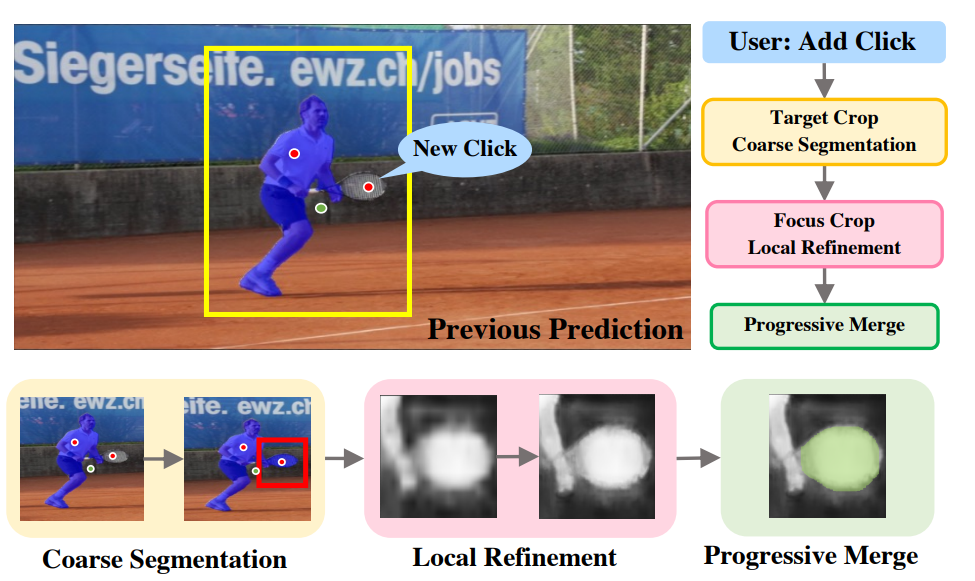
\includegraphics[width=12cm]{figuras/focalclick}}
		}{
			\Fonte{\cite{chen2022focalclick}}
		}
\end{figure}


\subsection{Interactive image segmentation based on multi-layer
random forest classifiers}\label{sec:superpixel-random-forest}

Neste trabalho, as autoras\cite{shan2023interactive} criam uma nova
técnica para segmentação interativa de imagens combinando uma
pré-segmentação usando superpixels e duas camadas de modelos random
forest para classificar o agrupamento entre os superpixels numa
máscara de segmentação resultante.


\section{Justificativas}\label{sec:justificativas}

Como mencionado na introdução, os algoritmos conhecidos de segmentação
de imagens possuem restrições pertinentes que podem dificultar o uso
das técnicas em alguns problemas, como imagens médicas e edição de
imagens.

Estes problemas são endereçados no desenvolvimento de uma nova técnica
de segmentação de imagens que explora outros novos ramos de
aprendizagem de máquina semi-supervisionada além das \gls{DNN}, neste
caso utilizando redes complexas e dinâmicas coletivas.

O campo de pesquisa de segmentação interativa também tem tido aumento
na publicação de artigos de relevância, em especial a publicação de
artigos com a palavra-chave GrabCut (tipo de algoritmo para
segmentação interativa), como pode ser visto na
Figura~\ref{fig:grabcut-papers}:

\begin{figure}[!h]
        \captionsetup{width=12cm}
		\Caption{\label{fig:grabcut-papers}
          Quantidade de publicações relevantes envolvendo grabcut de
          2004 a 2022}
		\centering
		\UFCfig{}{
			\fbox{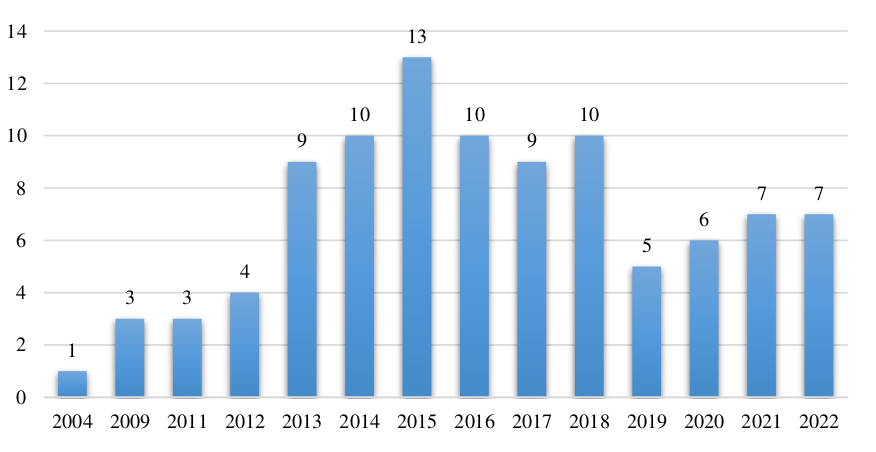
\includegraphics[width=12cm]{figuras/grabcut-papers}}
		}{
			\Fonte{\cite{wang2023review}}
		}
\end{figure}



\section{Objetivo Geral}\label{sec:objetivo-geral}

Desenvolver uma nova técnica de segmentação de imagens
semi-supervisionada que possa ser equiparável ao estado da arte, com
foco em segmentação interativa.

\section{Objetivos Específicos}\label{sec:objetivo-geral}

\begin{itemize}
\item Explorar técnicas de redes complexas e dinâmicas coletivas sobre
  o problema de segmentação de imagens.
\item Aplicar em casos variados de segmentação de imagens, como
  objetos comuns, carros.
\item Avaliar o impacto da segmentação por superpixel na segmentação final.
\item Desenvolver uma ferramenta para segmentação interativa
  utilizando o método de segmentação proposto.
\end{itemize}



% LocalWords:  transdutivo superpixel

	\chapter{OBJETIVOS}\label{cap:objetivos}

\begin{itemize}
\item Desenvolver uma nova técnica de segmentação de imagens que possa ser
equiparável ao estado da arte, como \textit{Mask R-CNN}, mas com menor
complexidade computacional e baixo número de anotação de dados.
\item Explorar técnicas de Redes Complexas e Dinâmicas Coletivas sobre
  o problema de segmentação de imagens.
\item Aplicar a técnica desenvolvida em casos de imagens médicas, como
  radiografias pulmonares.
\item Aplicar em casos variados de segmentação de imagens, como
  objetos comuns, carros.
\end{itemize}

	\chapter{FUNDAMENTAÇÃO TEÓRICA}\label{cap:fundamentacao-teorica}


Neste capítulo são apresentados vários conceitos e técnicas para fundamentar
o desenvolvimento do método proposto, descrito na seção~\ref{sec:teorica-egsis}.


\section{Segmentação interativa de imagens}\label{sec:segmentacao-interativa}

A segmentação interativa de imagens é um processo de divisão de uma
imagem digital em várias partes ou regiões, geralmente para tornar a
imagem mais fácil de analisar e processar~\cite{ramadan2020survey}. Este processo é `interativo'
porque envolve a entrada do usuário para ajudar a orientar ou refinar
o processo de segmentação.

\begin{figure}[h!]
        \captionsetup{width=12cm}
		\Caption{\label{fig:interactive-segmentation}
          O usuário marca anotações do fundo e do objeto a ser
          segmentado, então a segmentação interativa é realizada.
        }
		\centering
		\UFCfig{}{\fbox{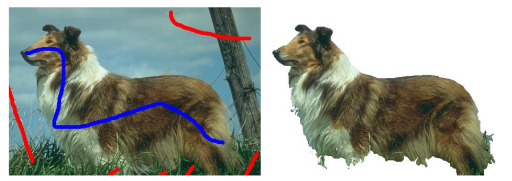
\includegraphics[width=12cm]{figuras/interactive-segmentation-2008}}}{\Fonte{\cite{duchenne2008segmentation}}}
\end{figure}
\FloatBarrier{}

De acordo com a figura~\ref{fig:interactive-segmentation}, na
segmentação interativa de imagens, o usuário pode selecionar regiões
de interesse, definir marcadores ou fazer anotações na imagem. Essas
entradas do usuário são então usadas para informar o algoritmo de
segmentação sobre como dividir a imagem. Por exemplo, o usuário pode
desenhar uma linha ao redor de um objeto de interesse, e o algoritmo
de segmentação irá então tentar dividir a imagem de tal forma que o
objeto de interesse seja isolado em sua própria região.

Este tipo de segmentação de imagem é útil em uma variedade de
aplicações, incluindo processamento de imagens médicas, visão
computacional, reconhecimento de padrões e muitos outros campos onde é
útil poder dividir uma imagem em regiões distintas com base em
critérios definidos pelo usuário.

\section{Aprendizado semi-supervisionado vs.\ transdução}\label{sec:teorica-aprendizado-semi-supervisionado}

Existem três principais categorias de aprendizado de máquina:
aprendizado supervisionado, aprendizado não supervisionado e
aprendizado semi-supervisionado. No aprendizado supervisionado durante
a etapa de treinamento existe uma base de dados totalmente rotulada,
no aprendizado não supervisionado não é disponibilizado nenhum
rotulamento dos dados. Enquanto isso, o aprendizado
semi-supervisionado está entre essas duas categorias.

O aprendizado semi-supervisionado é um método de aprendizado de máquina
que envolve o uso de um grande volume de dados não rotulados e um
pequeno volume de dados rotulados para treinar modelos de aprendizado
de máquina.

Formalmente, pode-se definir o aprendizado semi-supervisionado da seguinte maneira:

\begin{quote}
  Dado um conjunto de dados de treinamento
  $ \mathbf{X} = \{\vec{x_1}, \vec{x_2}, \ldots, \vec{x_n}\} $, tal que $ \vec{x_n} \in \mathbb{R}^d $,
  onde apenas um subconjunto  $ \vec{Y} = \{y_1, y_2, \ldots , y_m\} $ em que $ (m < n) $ tem rótulos
  correspondentes, o objetivo do aprendizado semi-supervisionado é usar
  tanto o conjunto de dados rotulado quanto o não rotulado para aprender
  a função $ f: \mathbf{X} \rightarrow \vec{Y} $ que pode prever o rótulo $ y $ para um novo
  exemplo $ \vec{x} $.
\end{quote}

O aprendizado semi-supervisionado é baseado na suposição de que os
dados não rotulados podem fornecer informações adicionais que podem
ser usadas para melhorar a precisão do modelo de aprendizado de
máquina. Isso é feito através de várias técnicas, como a propagação de
rótulos, na qual os rótulos são propagados dos dados rotulados para os
dados não rotulados, ou a aprendizagem auto-supervisionada, onde o
modelo é treinado para prever partes dos dados a partir de outras
partes.

Por outro lado, existe um diferente tipo de aprendizado
semi-supervisionado que não realiza a etapa de estimar a função $ f
$. Algoritmos que estimam essa função são descritos como indutivos,
pois após o treinamento, para classificar novos dados, realizam uma
inferência por indução ao aplicar a função estimada.

Em contraponto, existem algoritmos que não estimam tal função e apenas
realizam a inferência direta entre os dados rotulados disponíveis e os
não rotulados. Isso é chamado de transdução e um algoritmo bem
conhecido com essa característica é o classificador \gls{k-NN}.\@ Na
figura~\ref{fig:induction-vs-transduction} são ilustradas as
diferenças entre transdução e indução no processo de aprendizagem:


\begin{figure}[h!]
        \captionsetup{width=12cm}
		\Caption{\label{fig:induction-vs-transduction}
          No aprendizado transdutivo, a inferência em novos exemplos
          ocorre de maneira direta.
        }
		\centering
		\UFCfig{}{\fbox{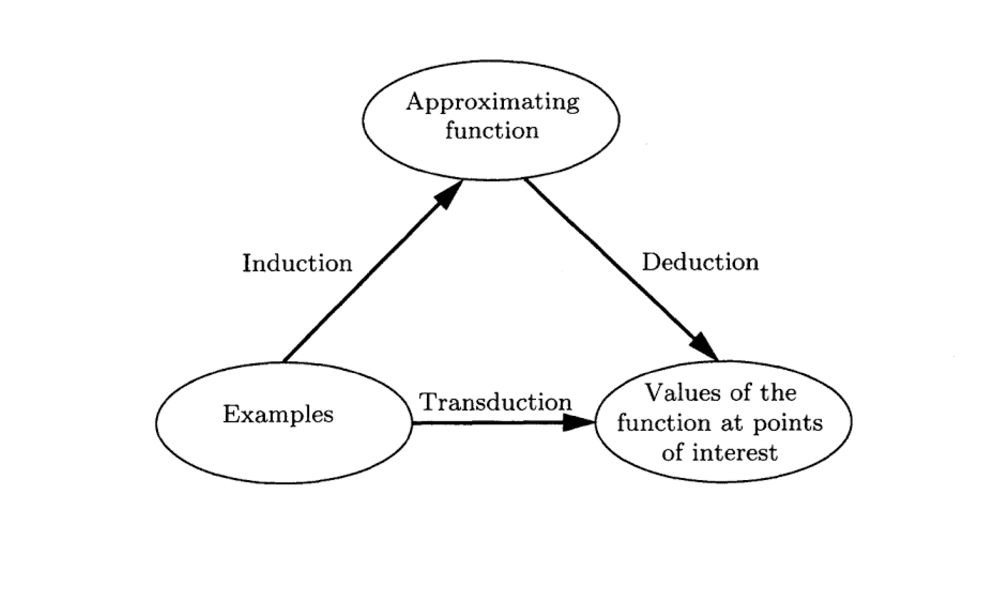
\includegraphics[width=12cm]{figuras/induction_vs_transduction}}}{\Fonte{\cite{vapnik1995}}}
\end{figure}


No texto~\cite{vapnik2006semi}, o criador do famoso algoritmo SVM,
estabelece uma profunda formalização dos problemas de aprendizado
semi-supervisionado e inferência transdutiva. No final do texto, ele declara
algumas reflexões sobre a solução de problemas em aprendizagem de
máquina. Em uma delas, ele diz que ao resolver um problema, não tente
resolver o problema geral como um passo intermediário, tente obter a
resposta que você precisa, mas não a mais geral. Por fim, Vapnik
deixa uma sugestão relevante:


\begin{displayquote}

  Do not estimate a function if you need to estimate values at given
  points. (Try to perform transduction, not induction.)

\end{displayquote}

Em tradução-livre: \blockquote{Não estime uma função se você precisa estimar
os valores em dados pontos. (Tente executar transdução, não
indução)}. Essa sugestão é uma evidência que reforça a motivação
deste trabalho. Ao desenvolver um algoritmo transdutivo pra
segmentação de imagens de maneira assistida, não é estimada uma função
geral como um passo intermediário, mas a segmentação é realizada
diretamente baseada nas rotulações iniciais que o usuário forneceu.


\section{Superpixels}\label{sec:teorica-superpixel}

Superpixels fazem parte de um grupo de algoritmos de clusterização em
processamento de imagens que ganhou popularidade nos últimos anos na
comunidade de visão computacional~\cite{SuperpixelSurvey2020}. Em vez
de processar uma imagem pixel por pixel, agrupam-se pixels vizinhos
semelhantes em uma entidade maior, conhecida como superpixel.

O conceito de superpixels foi introduzido para superar as limitações
do processamento pixel a pixel, que não leva em consideração a
estrutura global da imagem. Os superpixels, por outro lado, mantêm a
estrutura da imagem e reduzem a complexidade do processamento de
imagens, tornando-o mais eficiente.

Os superpixels são formados com base na similaridade dos pixels em
termos de cor, intensidade e localização na imagem. Eles são usados em
uma variedade de aplicações, incluindo segmentação de imagem,
rastreamento de objetos, reconhecimento de objetos, entre outros.

Em resumo, os superpixels são uma técnica eficaz para simplificar a
representação de uma imagem e aumentar a eficiência do processamento
de imagens, mantendo a informação visual importante.

Atualmente, já é possível encontrar muitas técnicas baseadas em
superpixels com diferentes características, complexidades
computacionais, métodos e eficiência. No
artigo~\cite{SuperPixelBenchmark2017}, é realizado um \textit{benchmark} com 15
algoritmos do tipo superpixel categorizados em três grupos: baseado em grafos,
baseado em otimização de gradiente e baseado em análise de
textura. Neste trabalho, é selecionado um dos mais simples: \gls{SLIC}.

\subsection{SLIC}\label{sec:teorica-superpixel-slic}


O algoritmo \gls{SLIC}~\cite{achanta2010slic} é um método para segmentação de imagens baseado
em superpixel, é um dos mais simples e pode ser visto como uma
variação do algoritmo de clusterização k-means expandindo o espaço
euclidiano ao incluir também o espaço de cores. Ele divide uma imagem
em segmentos menores, chamados superpixels, que compartilham
características semelhantes, como cor e textura.

Uma explicação passo-a-passo de como o SLIC funciona pode ser entendida
dessa maneira:

\begin{algorithm}[h!]
	\SetSpacedAlgorithm{}
	\caption{\label{alg:slic} SLIC}
	\Entrada{Imagem a ser segmentada}
    \Resultado{Matriz de superpixels}
	\Inicio{
      \begin{enumerate}

      \item \textbf{Inicialização}: O algoritmo começa selecionando alguns pixels na
        imagem como centros de superpixels. Esses centros são espaçados
        uniformemente pela imagem;

      \item \textbf{Atribuição}: Em seguida, para cada pixel na imagem, o algoritmo
        calcula a distância entre esse pixel e todos os centros de
        superpixels. A distância é calculada com base na cor (ou intensidade
        de níveis de cinza) e na proximidade espacial. O
        pixel é então atribuído ao superpixel cujo centro está mais próximo;

      \item \textbf{Atualização}: Depois que todos os pixels foram atribuídos a um
        superpixel, o algoritmo recalcula os centros de superpixels como a
        média de todos os pixels dentro de cada superpixel;

      \item O processo de atribuição e atualização é repetido várias vezes
        até que o algoritmo alcance a condição de convergência, ou seja, até
        que os centros de superpixels parem de mudar significativamente;

      \item O resultado final é uma segmentação da imagem em superpixels, onde
        cada superpixel é um grupo de pixels com características semelhantes.
    \end{enumerate}
   }
\end{algorithm}


Uma execução do SLIC é possível de ser visualizada a seguir:

\begin{figure}[h!]
        \captionsetup{width=12cm}
		\Caption{\label{fig:slic}
          Execução do algoritmo SLIC na fotografia de um gato.
        }
		\centering
		\UFCfig{}{\fbox{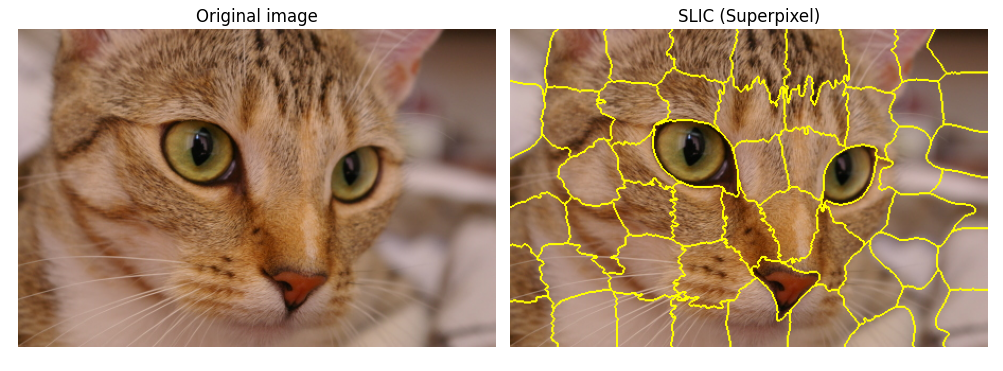
\includegraphics[width=12cm]{figuras/slic}}}{\Fonte{\fonteautorscikit}}
\end{figure}

O algoritmo \gls{SLIC} possuí três hiperparâmetros: \textit{segments}, sigma e \textit{compactness}.

\begin{enumerate}
\item \textbf{Segments}: Número de superpixels que será usado para
  segmentar a imagem.
\item \textbf{Sigma}: Este parâmetro é usado para suavizar a imagem antes da
segmentação. Um valor maior de sigma resultará em uma imagem mais
suave, o que pode ajudar a reduzir o ruído e os detalhes finos. No
entanto, um valor muito alto pode resultar em perda de detalhes
importantes.
\item \textbf{Compactness} Este parâmetro controla o equilíbrio entre a coerência
de cor e a proximidade espacial na formação de superpixels. Um valor
maior de compactness fará com que os superpixels sejam mais
quadrados, enquanto um valor menor fará com que os superpixels
sigam mais de perto os limites da imagem. Portanto, a compactness pode
ser ajustada para obter superpixels que são mais representativos da
estrutura da imagem.
\end{enumerate}


\section{Geração de redes complexas}\label{sec:teorica-redes-complexas}

Redes complexas são grafos de alta complexidade. Existem variados
algoritmos para geração de redes complexas
~\cite{ComplexNetworksSurvey2007}. Redes complexas podem ser usadas
como um domínio de dados para realizar tarefas como classificação de
imagens~\cite{ComplexNetworksImageClassification2015}, segmentação de
imagens, identificação de comunidades e também extração de
características~\cite{JarbasComplexNetworks2020}.

Neste trabalho, o uso de redes complexas é realizado de uma maneira
acoplada ao algoritmo de clusterização inicial da imagem (superpixel). Nesse
cenário, cada superpixel gerado na imagem é um vértice e as arestas
são gerados com base na vizinhança.

Apesar de considerar o tema como redes complexas, esse cenário em
particular gera um grafo planar pela maneira como as arestas são
criadas. Por outro lado, seria possível também modificar a geração da
rede complexa para considerar as arestas do grafo baseado num raio
parametrizado de superpixel em relação a um \textit{treshrold} e
selecionar as \gls{k-NN} similares como arestas válidas.

Essa etapa de geração da rede complexa é crucial para a execução da
dinâmica coletiva explorada na seção~\ref{sec:teorica-lcu}, que é um dos
pontos centrais deste trabalho. Na figura~\ref{fig:complex-networks},
um exemplo de geração de rede complexa é apresentado conectado com a
ilustração~\ref{fig:slic}, ao executar o algoritmo SLIC.\@

\begin{figure}[t]
        \captionsetup{width=12cm}
		\Caption{\label{fig:complex-networks}
          Geração de rede complexa baseado nos superpixels.
        }
		\centering
		\UFCfig{}{\fbox{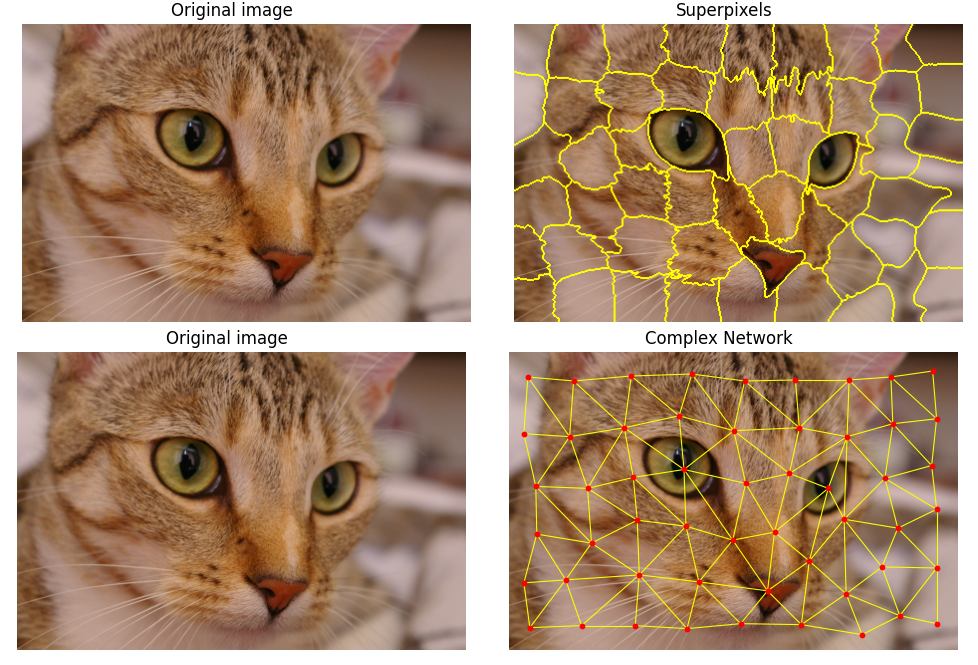
\includegraphics[width=12cm]{figuras/complex-networks}}}{\Fonte{\fonteautorscikit}}
\end{figure}
\FloatBarrier{}

\section{Extração de características}\label{sec:extracao-caracteristicas}

\subsection{Matriz de co-ocorrências}\label{sec:teorica-matriz-co-ocorrencia}

O método de extração de características da matriz de
co-ocorrências~\cite{haralick1979statistical} é uma técnica utilizada em
processamento de imagem e visão computacional para extrair
características texturais de uma imagem.

Formalmente, uma matriz de co-ocorrência $C$ é definida sobre uma imagem
$I$, para um deslocamento $\Delta x, \Delta y$, como:

\begin{equation}\label{eq:comatrix}
  C_{\Delta x, \Delta y}(i,j) = \sum_{x=1}^n\sum_{y=1}^m
  \begin{cases} 1, & \text{if }I(x,y)=i\text{ e }I(x+\Delta x, y+\Delta y)=j
               \\ 0, & \text{caso contrário}
  \end{cases}
\end{equation}

Na equação~\ref{eq:comatrix} $C_{\Delta x, \Delta y}(i,j)$ é o número de vezes
que o par de pixels com intensidades $i$ e $j$ ocorre em dois pixels
separados pelas distâncias (horizontal e vertical) na imagem $I$.

A matriz de co-ocorrência é tipicamente normalizada dividindo cada
elemento pelo número total de pares de pixels na imagem, resultando em
uma matriz de probabilidade de co-ocorrência.

A partir desta matriz, várias características texturais podem ser
extraídas, como contraste, correlação, energia e homogeneidade. Estas
características podem ser usadas para tarefas como classificação de
textura, segmentação de imagem, entre outros. Após a aplicação do
método em cada canal RGB da imagem, são extraídas cinco estatísticas: média,
mediana, variância, desvio padrão e 25-quantis. Então as
características são concatenadas um vetor de características de 15 dimensões.

\subsection{Filtros de Gabor}\label{sec:filtros-gabor}

Os filtros de Gabor~\cite{daugman1988complete} são uma família de filtros
de convolução usados principalmente na análise de texturas e na visão
computacional para a extração de características. Eles são nomeados em
homenagem a Dennis Gabor, o físico que ganhou o Prêmio Nobel por sua
invenção e desenvolvimento do método holográfico.

Os filtros de Gabor são essencialmente filtros passa-banda orientados
e localizados no espaço de frequência. Eles são muito úteis para a
extração de características porque têm propriedades ótimas de
localização no espaço e na frequência, o que os torna muito adequados
para a captura de características locais e direcionais em uma imagem.

Os filtros de Gabor são definidos por duas funções: uma função
gaussiana (para o domínio espacial) e uma função harmônica complexa
(para o domínio da frequência). A função gaussiana serve para limitar
a aplicação do filtro a uma pequena região da imagem (localização
espacial), enquanto a função harmônica complexa permite capturar
características em uma determinada orientação. Na
figura~\ref{fig:gabor-filters} são ilustrados variações dos
filtros de Gabor com diferentes parâmetros e a convolução resultante.

\begin{figure}[!h]
        \captionsetup{width=12cm}
		\Caption{\label{fig:gabor-filters}
          Filtros de Gabor variando a angulação $\theta$ e a convolução resultante.
        }
		\centering
		\UFCfig{}{\fbox{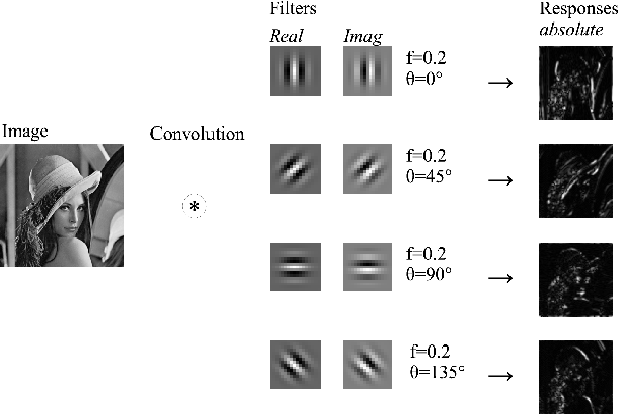
\includegraphics[width=12cm]{figuras/gabor-filters}}}{\Fonte{\cite{Kmrinen2012GaborFI}}}
\end{figure}
\FloatBarrier{}

A operação de convolução entre uma imagem qualquer $ x $ e um filtro de
Gabor $ k $, pode ser dada pela seguinte equação:

\begin{equation}
  (y * k)(i, j) = \sum_{m} \sum_{n} x(i-m, j-n) k(m, n)
\end{equation}

A extração de características usando filtros de Gabor geralmente
envolve a convolução da imagem com um conjunto de filtros de
Gabor. Cada filtro é sensível a características de uma determinada
escala e orientação. A resposta do filtro pode então ser usada como
uma representação da presença de tais características na imagem.

Neste trabalho, são gerados 16 filtros de Gabor que foram avaliados
experimentalmente com variados parâmetros. Após a aplicação do filtro
em cada canal RGB da imagem, são extraídos cinco estatísticas: média,
mediana, variância, desvio padrão e 25-quantis. Com isso, todas as
cinco estatisticas dos 16 filtros aplicados em cada um dos três canais
são concatenadas num único vetor de características resultante com 240
($16 \times 5 \times 3$) dimensões, pois é o resultado.

\section{Métricas de similaridade}\label{sec:teorica-metricas-de-similaridade}


Métricas de similaridade neste trabalho são calculadas com o propósito
de comparar a similaridade entre os vetores de características dos
superpixels. Para as técnicas de extração de características descritas
na seção~\ref{sec:extracao-caracteristicas}, cada técnica se comportou
melhor com uma métrica de similaridade diferente.

Uma função de similaridade entre dois vetores de características
retorna um valor maior quando os vetores são similares e quanto mais
diferentes sejam, mais a similaridade tende a zero.

A estrutura de uma métrica de similaridade pode ser criada a partir de
uma métrica de distância. Neste trabalho, são exploradas duas métricas de
similaridades a partir das seguintes métricas de distância: distância
euclidiana e distância de manhattan.

A distância euclidiana é o módulo da reta que conecta dois pontos no
espaço. A distância de manhattan é a soma da diferença absoluta entre
dois pontos para cada dimensão. Na
figura~\ref{fig:manhattan-vs-euclidean} é ilustrado a disposição de
dois pontos $ x $ e $ y $ no espaço euclidiano com os módulos de
segmento de reta usados para compor a distância de cada métrica.

\begin{figure}[!h]
        \captionsetup{width=8cm}
		\Caption{\label{fig:manhattan-vs-euclidean}
          Visualização da distância de manhattan e distância euclidiana.
        }
		\centering
		\UFCfig{}{\fbox{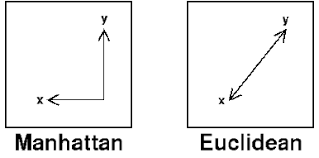
\includegraphics[width=8cm]{figuras/manhattan-vs-euclidean}}}{\Fonte{\cite{Singh2019}}}
\end{figure}
\FloatBarrier{}

Para as equações das distâncias, tem-se a seguinte equação para a
distância euclidiana:

\begin{equation}\label{eq:euclidian-distance}
ed(\vec{x}, \vec{y}) = \sqrt{{(y_1-x_1)}^2 + {(y_2-x_2)}^2 + \cdots + {(y_n-x_n)}^2}
\end{equation}

Para a distância de manhattan, tem-se a seguinte equação:

\begin{equation}\label{eq:manhattan-distance}
md(\vec{x}, \vec{y}) = |y_1-x_1| + |y_2-x_2| + \cdots + |y_n-x_n|
\end{equation}

\subsection{Similaridade Euclidiana Exponencial}\label{sec:teorica-similaridade-euclidiana}

Para a técnica de extração de característica de matrizes de co-ocorrência,
detalhada na seção~\ref{sec:teorica-matriz-co-ocorrencia}, a métrica de
similaridade que obteve os melhores resultados foi a distância
euclidiana pelo inverso da exponencial. A equação é definida como:

\begin{equation}\label{eq:euclidian-similarity}
  ed\_sim(\vec{x}, \vec{y}) = \dfrac{1}{e^{ed(\vec{x}, \vec{y})}}
\end{equation}

\subsection{Similaridade de Manhattan Logarítmica}\label{sec:teorica-similaridade-manhattan}

Para a técnica envolvendo filtros de Gabor, a distância entre os
vetores de características tiveram valores tão altos que ao usar a
similaridade euclidiana (exponencial ou não), maior parte dos valores
chegavam a zero. Por esse motivo, o uso da conversão para o domínio
logarítmico foi usado para suavizar o crescimento exagerado dos
valores, obtendo bons resultados. A definição para essa equação de
similaridade segue a seguir:

\begin{equation}\label{eq:manhattan-similarity}
  md\_sim(\vec{x}, \vec{y}) = \dfrac{1}{1 + \ln(1 + md(\vec{x}, \vec{y}))}
\end{equation}

Na equação~\ref{eq:manhattan-similarity}, os valores $1$ adicionados
ao denominador foram necessários para evitar uma possível divisão por
zero e logarítmo de zero, ambas operações que são indefinidas na
matemática.


\section{LCU}\label{sec:teorica-lcu}

O algoritmo \gls{LCU} foi desenvolvido por um
brasileiro~\cite{VerriNetworkUnfoldingMap2018}, é uma dinâmica
coletiva baseada em propagação de rótulos numa rede complexa. Essa
dinâmica coletiva é modelada como um sistema dinâmico com geração de
partículas de rotulação nas suas fontes (os vértices rotulados).

Esse algoritmo possui critérios de sobrevivência das partículas
inspirado em comportamentos da natureza e sociedade. Por exemplo, o
hiperparâmetro $ \lambda $ do algoritmo denota um fator de competição entre
0 e 1 sobre o dificuldade que as partículas terão ao trafegar nos
vértices, tornando a sobrevivência delas mais difícil ao percorrer o
grafo. Para esse parâmetro, 0 significa um passeio aleatório no grafo,
1 significa máxima competitividade. Embora as partículas nasçam nos
vértices, a competição por dominação acontece nas arestas. No final, o
vértice será marcado com o novo rótulo baseado no tipo de partícula
que mais conseguiu dominar arestas desse vértice.

Nesse caso particular, a implementação proposta neste trabalho é
ligeiramente diferente da proposta originalmente, pois a rede complexa
no cenário que o autor propõe as arestas não possuem peso. Uma
modificação é realizada para incluir a similaridade de imagem entre
dois superpixels, dessa maneira é criado um fator de aumento da
probabilidade das partículas visitarem os nós mais promissores
(texturas mais similares). Como discutido na
seção~\ref{sec:teorica-aprendizado-semi-supervisionado}, esse cenário
de aprendizado é semi-supervisionado transdutivo: poucos rótulos estão
disponíveis e nenhuma função de inferência é estimada. A inferência
acontece diretamente entre os pontos rotulados e os não-rotulados.


\begin{figure}[!h]
\centering
    \captionsetup{width=14cm}
    \Caption{\label{fig:lcu-execution}
      Rede complexa para execução da dinâmica LCU.\@ Anotação
      parcial em~(\subref{fig:lcu-partial}) e resultado final em~(\subref{fig:lcu-done})
    }

    \begin{subfigure}[b]{0.45\textwidth}
    \centering
    \UFCfig{}{\fbox{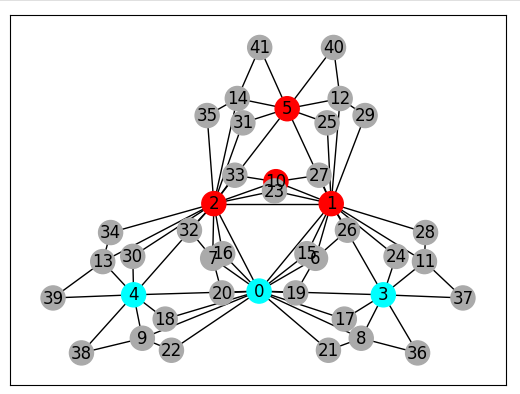
\includegraphics[width=7cm]{figuras/lcu-partial}}}
    \caption{\label{fig:lcu-partial}}
    \end{subfigure}
\quad
    \begin{subfigure}[b]{0.45\textwidth}
    \centering
    \UFCfig{}{\fbox{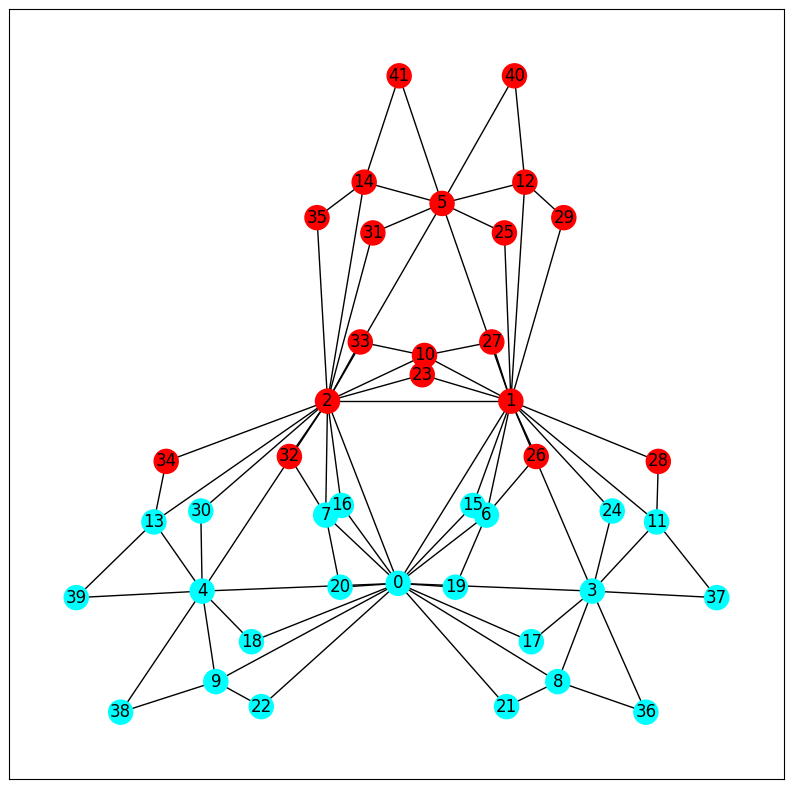
\includegraphics[width=7cm]{figuras/lcu-done}}}
    \caption{\label{fig:lcu-done}}
    \end{subfigure}
    {\Fonte{\fonteautor}}
\quad
\end{figure}
\FloatBarrier{}


Na figura~\ref{fig:lcu-execution}, é possível ver a execução do
algoritmo numa rede complexa densa aleatória, no início há alguns
poucos vértices anotados em azul e vermelho. No final da execução os
rótulos são propagados semanticamente baseado na disputa entre as
partículas para dominar arestas, e por fim, marcar os vértices
dominados por aquela classe.

Em mais detalhes, durante uma única iteração do sistema na
figura~\ref{fig:lcu-iteration}, pode-se visualizar o passeio das
partículas entre as fontes de partículas (vértices rotulados) verde e
vermelho. Algumas não sobreviveram ao processo, outras se mantiveram
no sistema. Na última imagem, uma contagem do número de partículas por
classe que passaram pelas arestas pode ser vista.


\begin{figure}[h!]
        \captionsetup{width=8cm}
		\Caption{\label{fig:lcu-iteration}
          Iteração do sistema LCU em um grafo planar.
        }
		\centering
		\UFCfig{}{\fbox{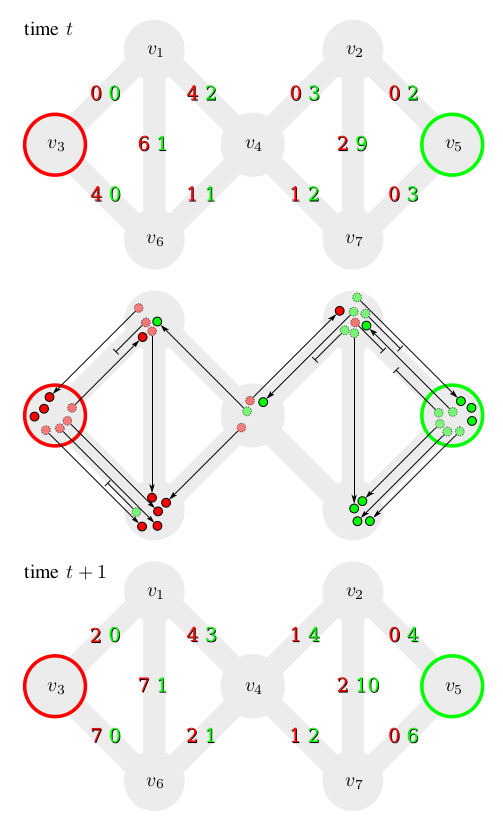
\includegraphics[width=8cm]{figuras/lcu-iteration}}}{\Fonte{\cite{VerriNetworkUnfoldingMap2018}}}
\end{figure}


\subsection{Modelagem matemática LCU com grafo ponderado}\label{sec:lcu-math}

Considera-se uma rede complexa expressada por um simples grafo
ponderado não-direcionado $G = (\mathcal{V}, \mathcal{E})$, onde $\mathcal{V}$ é o conjunto de
vértices e $\mathcal{E} \subset \mathcal{V} \times \mathcal{V}$ é o conjunto de arestas. A rede possui
$\left|\mathcal{V}\right| = l + u$ vértices que podem ser representações de
dados rotulados ($ l $) ou não-rotulados ($ u $). Os vértices anotados
podem ter um rótulo $y_i = \{1, \ldots, C\}$, em que $C$ é o número total de
classes, além disso possuem um vetor de características $\vec{x_i}$ da
representação daquele dado. A rede é representada por uma matriz de
adjacência $A = (a_{ij})$, onde $a_{ij} =a_{ji} =
similarity(\vec{x_i}, \vec{x_j})$, na qual as arestas possuem um peso
que se refere à similaridade entre os vetores de características
representados pelos vértices. Nessa situação, supõe-se que $l << u$,
ou seja, há muito mais dados não-rotulados do que rotulados, na qual
caracteriza-se um cenário para aprendizado semi-supervisionado.

Os vértices rotulados são chamados de fontes, que geram partículas com
a classe que responde ao vértice. Partículas que alcançam um vértice fonte
com classe diferente são eliminados automaticamente do sistema.

O sistema dinâmico não-linear $X(t)$ que representa o \gls{LCU} é definido
matematicamente como:

\begin{equation}\label{eq:lcu-x}
  X(t):=\left[\begin{array}{c}
    \mathbf{n}^c(t)={\left[n_i^c(t)\right]}_i \\
    N^c(t)={\left(n_{i j}^c(t)\right)}_{i, j} \\
    \Delta^c(t)={\left(\delta_{i j}^c(t)\right)}_{i, j}
\end{array}\right]
\end{equation}

\noindent
Em que $ \mathbf{n}^c(t)$ é um vetor linha cujo elementos $n_i^c(t)$
representam a população de partículas com rótulo $c$ em cada vértice
$v_i$ no tempo $t$. Os elementos $n_{i j}^c(t)$ representam o número
de partículas da classe $c$ que se movem do vértice $v_i$ para $v_j$ no
tempo $ t $, enquanto $\delta_{i j}^c(t)$ representa a movimentação
acumulada de partículas da classe $c$ entre a aresta $(i, j)$ no tempo
$t$.

A função determinística de evolução do sistema dinâmico é definida
por:

\begin{equation}\label{eq:lcu-phi-evolution}
  \phi:\left\{\begin{array}{l}
    \mathbf{n}^c(t+1)= P^c(X(t)) \times \mathbf{n}^c(t) +\mathbf{g}^c(X(t)) \\
    N^c(t+1)=\operatorname{diag} \mathbf{n}^c(t) \times P^c(X(t)) \\
    \Delta^c(t+1)=\Delta^c(t)+N^c(t+1),
  \end{array}\right.
\end{equation}

Entre as funções ainda não definidas na função de evolução, destaca-se a de
probabilidade de sobrevivência das partículas $P^c(X(t))$, na qual os
elementos dessa matriz são definidos como:

\begin{equation} \label{eq:lcu-probability}
  p_{i j}^c(X(t)):= \begin{cases}0 & \text { se } v_j \in \mathcal{L} \text { e
                                     } y_j \neq c, \\
    \frac{a_{i j}}{\deg v_i}\left(1-\lambda \sigma_{i
    j}^c(X(t))\right) & \text { do contrário }\end{cases}
\end{equation}
\noindent
Em que ${\deg v_i}$ o grau do vértice (número de arestas
conectadas) e variável $\sigma_{i j}^c$ define-se como:

\begin{equation}\label{eq:lcu-sigma}
\begin{aligned}
\sigma_{i j}^c(X(t)):= \begin{cases}1-\frac{n_{i j}^c(t)+n_{j i}^c(t)}{S} & \text { se } S>0, \\
1-\frac{1}{C} & \text { do contrário, }\end{cases} \\
\text { sendo } S=\sum_{q=1}^C n_{i j}^q(t)+n_{j i}^q(t) .
\end{aligned}
\end{equation}

A modificação dessa dinâmica coletiva em relação à proposta original
em~\cite{VerriNetworkUnfoldingMap2018} é realizada em $a_{ij}$,
enquanto no trabalho original o grafo é não-ponderado e, portanto,
todas as arestas possuem valor unitário. Neste trabalho a aresta representa um
valor de similaridade entre os vetores de características anexados ao
vértice $v_i$ e $v_j$, dessa maneira aumentando a probabilidade de
sobrevivência de partículas que se movimentam por arestas com maior
similaridade.

A última função $\mathbf{g}^c(X(t))$ representa a geração de
partículas nos vértices fontes no tempo $t$, e é definida como:

\begin{equation}\label{eq:lcu-generation}
  \begin{aligned}
    g_i^c(X(t)) &:=\rho_i^c \max \left\{0, \sum_{j=1}^{\left| \mathcal{V} \right|}(\mathbf{n}_{j}^c(0) - \mathbf{n}_{j}^c(t))\right\} \\
    \rho_i^c &:= \begin{cases}\frac{\deg v_i}{\sum_{v_j \in \mathcal{G}^c}
      \deg v_j} & \text { se } v_i \in \mathcal{G}^c, \\ 0 & \text {
                                                               do contrário }\end{cases}
  \end{aligned}
\end{equation}

Na equação~\ref{eq:lcu-generation}, $\mathcal{G}^c = \{v_i |v_i \in \mathcal{L}, y_i = c\}$
é o conjunto de fontes de partículas que pertencem à classe $c$ e $\mathcal{L}$
é o conjunto dos vértices rotulados.


Após alcançar a iteração máxima de um valor escolhido para $ \tau $, é possível
dividir a rede complexa em sub-grafos, primeiramente agrupando as
arestas por maior dominação de classe:

\begin{equation}\label{eq:lcu-edges-by-class}
  \mathcal{E}^c(t):=\left\{(i, j) \mid \underset{q}{\arg \max }\left(\delta_{i j}^q(t)+\delta_{j i}^q(t)\right)=c\right\}
\end{equation}

E, então, define-se o grafo por classe $c$ como:

\begin{equation}\label{eq:lcu-subnetworks}
  G^c(t):=\left(\mathcal{V}, \mathcal{E}^c(t)\right)
\end{equation}

Por fim, as redes $ G^c(\tau) $ são usadas para classificação dos
vértices. São atribuídos os rótulos $y_j \in \{1, \ldots, C\}$ para cada
vértice não-rotulado com a informação provida pela rede $G^c$.  O
rótulo $y_j$ é atribuído baseado na densidade das arestas na sua
vizinhaça. Formalmente, escrito como:

\begin{equation}\label{eq:lcu-vertex-classification}
y_j = \underset{c \in \{1, \ldots, C\}}{\arg \max }\left| \mathcal{E}(\mathcal{N}_{c,j}) \right|
\end{equation}
\noindent
Em que ${\mathcal{N}_{c,j}}$ são as arestas da vizinhança do vértice $j$ que
foram dominadas por párticulas da classe $c$. Na
figura~\ref{fig:lcu-classification}, é ilustrada a dinâmica coletiva
aplicada em uma rede complexa de formato similar a duas bananas. A
ilustração está dividida em quatro etapas: (a) inicialização com 6
vértices rotulados, 3 para cada classe, vértices pretos não estão
rotulados; (b) 4 iterações do sistema, com as arestas coloridas
sendo dominadas por particulas, enquanto as cinzas ainda não foram
dominadas; (c) 20 iterações, todo o grafo foi percorrido; (d) a
classificação dos vértices pela classe correspondente que obteve maior
dominação.

\begin{figure}[h!]
        \captionsetup{width=12cm}
		\Caption{\label{fig:lcu-classification}
          Execução em quatro fases da dinâmica coletiva LCU.\@
        }
		\centering
		\UFCfig{}{\fbox{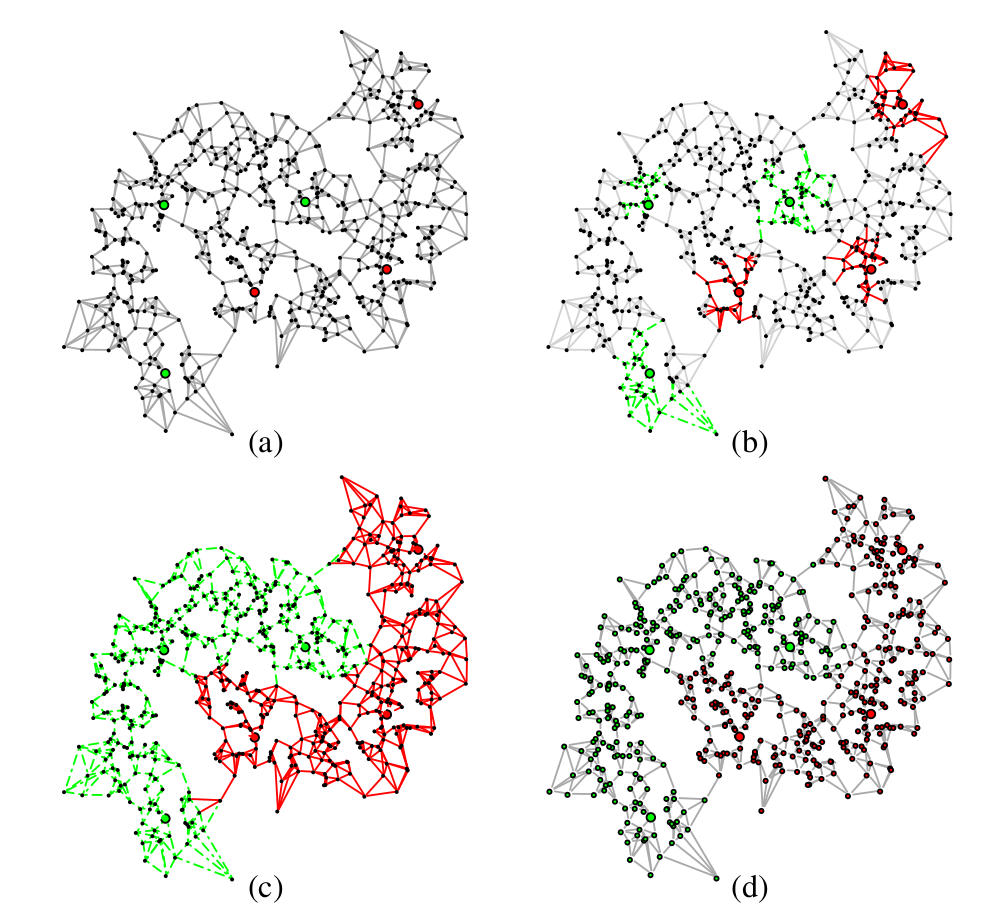
\includegraphics[width=12cm]{figuras/lcu-classification}}}{\Fonte{\cite{VerriNetworkUnfoldingMap2018}}}
\end{figure}

\section{EGSIS}\label{sec:teorica-egsis}

O algoritmo \gls{EGSIS} é a técnica de segmentação de imagens proposta
proposta neste trabalho. Todas as seções anteriores da fundamentação
teórica foram introduzidas para explicar o funcionamento dessa técnica
que será descrita nesta seção.

O modelo \gls{EGSIS} permite a execução de uma segmentação transdutiva
de imagens na presença de uma rotulação parcial da imagem. Essa
técnica possui etapas flexíveis para refinamento e otimização, quanto
a método de extração de características, quantidade de superpixels,
função de similaridade, entre outros.

Ao considerar as características do algoritmo LCU explicada na
seção~\ref{sec:teorica-lcu}, esse algoritmo também pode ser usado para
aprendizado semi-supervisionado multi-classe.

O ponto central desse método de segmentação é realizar uma
transformação do domínio da imagem para uma rede complexa que seja
compatível com a dinâmica coletiva \gls{LCU}. Para isso, uma
pré-segmentação é realizada usando superpixels através do algoritmo
SLIC.\@ Os rótulos iniciais da imagem são propagados aos superpixels
baseado numa votação: a classe que tiver maior números de pixels
rotulados, atribui-se aquela classe ao superpixel.

Ao obter os superpixels e os rótulos iniciais, é construída uma rede
complexa onde os vértices representam os superpixels e as arestas a
vizinhança com grau de similaridade entre os superpixels. Para
calcular a similaridade de cada aresta, primeiro é executado para cada
superpixel o método de extração de características selecionado, que
nesse caso pode ser filtros de Gabor ou matrizes de co-ocorrência,
então calcula-se a similaridade entre os superpixels com uma métrica
de similaridade selecionada.

Nessa etapa, a rede complexa é preparada para execução do sistema
dinâmico \gls{LCU} a fim de propagar os rótulos no grafo. No final da
execução do \gls{LCU}, é reconstruída uma máscara de segmentação
baseado nas rotulações dos vértices restantes em cada superpixel
não-rotulado. Por fim, obtém-se uma matriz de labels relacionando
cada pixel ao rótulo de segmentação desejado.

No Algoritmo~\ref{alg:egsis} são descritos as etapas do funcionamento
geral do método.

\begin{algorithm}[h!]
	\SetSpacedAlgorithm{}
	\caption{\label{alg:egsis} EGSIS}
	\Entrada{Imagem, rotulações parciais}
    \Resultado{Imagem segmentada}
	\Inicio{
      Inicializa os hiperparâmetros do modelo \gls{EGSIS}\;
      Segmenta a imagem em $n$ superpixels usando \gls{SLIC}\;
      Realiza a construção da rede complexa baseado nos superpixels\;
      Atribui os superpixels rotulados baseado na anotação parcial\;
      Calcula o vetor de características para cada superpixel\;
      Calcula a similaridade entre superpixels da vizinhança\;
      Executa a dinâmica LCU sobre a rede complexa gerada\;
      Reconstrói a máscara de segmentação com base nos vértices rotulados\;
   }
\end{algorithm}
\FloatBarrier{}

A seguir uma ilustração da execução do algoritmo em algumas etapas. Na
figura~\ref{fig:egsis-init}, são observadas duas etapas sendo
realizadas: na imagem (\subref{fig:egsis-superpixels}) a segmentação
por superpixels, na imagem (\subref{fig:egsis-complex-networks}) a rede
complexa gerada através dos superpixels.


\begin{figure}[!h]
\centering
    \captionsetup{width=14cm}
    \Caption{\label{fig:egsis-init}
      Construção de superpixels e a rede complexa no modelo EGSIS.\@
    }

    \begin{subfigure}[b]{0.45\textwidth}
    \centering
    \UFCfig{}{\fbox{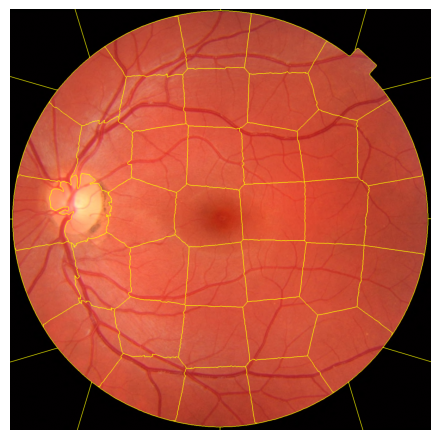
\includegraphics[width=7cm]{figuras/egsis-superpixels}}}
    \caption{\label{fig:egsis-superpixels}}
    \end{subfigure}
\quad
    \begin{subfigure}[b]{0.45\textwidth}
    \centering
    \UFCfig{}{\fbox{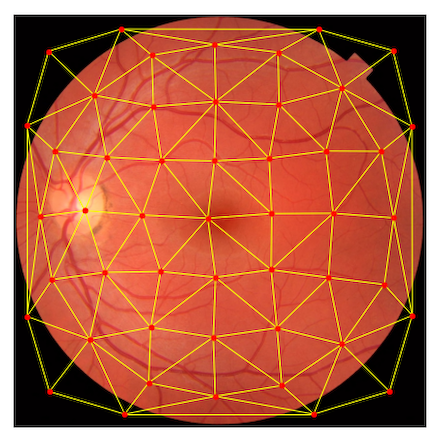
\includegraphics[width=7cm]{figuras/egsis-complex-networks}}}
    \caption{\label{fig:egsis-complex-networks}}
    \end{subfigure}
    {\Fonte{\fonteautorscikit}}
\quad
\end{figure}
\FloatBarrier{}



Na figura~\ref{fig:egsis-lcu}, há alguns superpixels
anotados em azul e vermelho, e uma segmentação em duas classes. Na outra
imagem, é ilustrado o resultado após a continuação da
execução. Perceba que boa parte da imagem foi segmentada corretamente, mas houve
alguns erros visíveis.

\begin{figure}[!h]
\centering
    \captionsetup{width=14cm}
    \Caption{\label{fig:egsis-lcu}
      Etapa do método EGSIS para propagar rótulos iniciais através do
      sistema dinâmico LCU.\@
    }

    \begin{subfigure}[b]{0.45\textwidth}
    \centering
    \UFCfig{}{\fbox{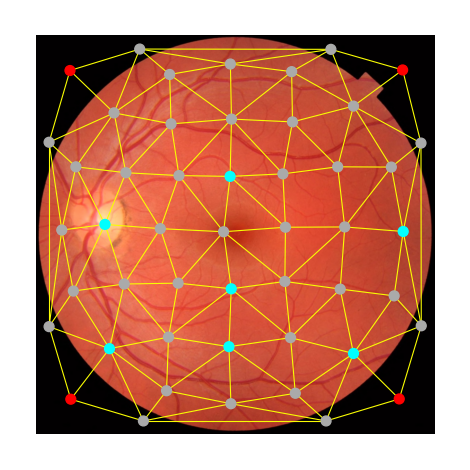
\includegraphics[width=7cm]{figuras/egsis-partial-labeled}}}
    \caption{\label{fig:egsis-partial-labeled}}
    \end{subfigure}
\quad
    \begin{subfigure}[b]{0.45\textwidth}
    \centering
    \UFCfig{}{\fbox{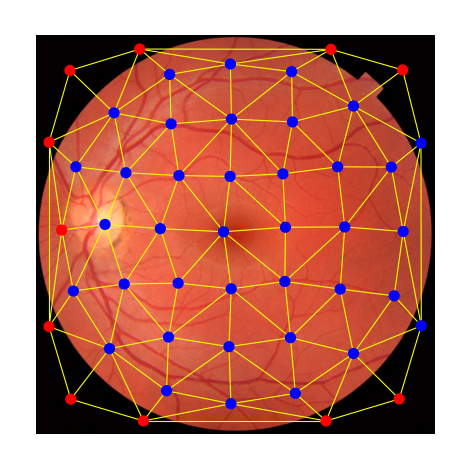
\includegraphics[width=7cm]{figuras/egsis-execution}}}
    \caption{\label{fig:egsis-execution}}
    \end{subfigure}
    {\Fonte{\fonteautorscikit}}
\quad
\end{figure}
\FloatBarrier{}

Por fim, obtém-se a seguinte máscara de segmentação ao atribuir os
rótulos dos vértices para os superpixels iniciais, assim sendo
possível reconstruir uma máscara de segmentação como ilustrado na
figura~\ref{fig:egsis-mask}.

\begin{figure}[h!]
        \captionsetup{width=12cm}
		\Caption{\label{fig:egsis-mask}
          Máscara de segmentação final e a imagem original.\@
        }
		\centering
		\UFCfig{}{\fbox{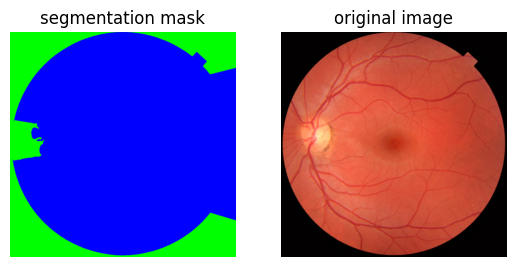
\includegraphics[width=12cm]{figuras/egsis-segmentation-mask}}}{\Fonte{\fonteautorscikit}}
\end{figure}

	\chapter{Justificativas}\label{cap:justificativas}

Como mencionado na introdução, os algoritmos conhecidos de segmentação
de imagens possuem restrições pertinentes que podem dificultar o uso
das técnicas em alguns problemas, como imagens médicas e edição de
imagens. Na seção \textit{revisão biblográfica} são mencionadas propriedades
pertinentes dos algoritmos propostos, como, por exemplo, possuirem complexidade
computacional linear.

Estes problemas são endereçados no desenvolvimento de uma nova técnica
de segmentação de imagens que explora outros novos ramos de
aprendizagem de máquina semi-supervisionada além das \gls{DNN}, neste
caso utilizando redes complexas e dinâmicas coletivas. Parte do
trabalho que tem sido desenvolvido em parceria com o \gls{ITA} no
projeto DNAYA\cite{DnayaMotivation}, como por exemplo a dinâmica coletiva \gls{LCU}.

Vale mencionar que, considerando a situação de pandemia que vive-se
desde 2020 com o COVID-19, a construção de tecnologias que facilitam o
diagnóstico de doenças respiratórias com auxílio de radiografias
pulmonares tem se tornado uma linha de pesquisa ainda mais relevante.

    \chapter{Trabalhos Relacionados}\label{cap:trabalhos-relacionados}

Técnicas de segmentação de imagens com o paradigma semi-supervisionado
estão em foco atualmente no campo médico, como pode ser visto em
~\cite{LuoSemiSupervised2021}. Nesse artigo, uma das grandes motivações
de os autores utilizarem uma técnica semi-supervisionada
está relacionado com a dificuldade de anotação de dados no ambiente
hospitalar, requisito para utilizar técnicas mais robustas como
\textit{Mask R-CNN}.

Em relação ao tópico de redes complexas e dinâmicas coletivas, é
possível mencionar o trabalho feito com o algoritmo \gls{LCU}
~\cite{VerriNetworkUnfoldingMap2018} no qual os principais conceitos
sobre resolução de problemas de aprendizagem de máquina
semi-supervisionada são explorados em detalhes como uma dinâmica de
competição de partículas na relação vértice-arestas de um grafo
não-direcionado. Este método de aprendizagem é transdutivo, portanto,
difere dos métodos indutivos, como é o caso de Redes Neurais. Além
disso, esse algoritmo tem complexidade computacional linear em relação
à quantidade de classes, arestas e vértices.

Para ilustrar uma possível ideia de segmentação de imagens, ao
considerar um algoritmo que faça uma transformação do domínio de
imagem para um grafo, é possível estabelecer uma relação na qual os
vértices representam parte da imagem como um \textit{superpixel}
~\cite{SuperpixelSurvey2020}, ou seja, um grupo de subpixels da
imagem. Na Figura~\ref{fig:segmentation-superpixel} é apresentado um
exemplo de segmentação usando superpixels. Algoritmos de superpixel
são não-supervisionados em geral, portanto possuem suas limitações
quanto ao resultado esperado pelo usuário \textendash\hfill logo
difícil de ser aceito em aplicações médicas nas quais a opinião do
especialista é de alta relevância para o resultado final.

\begin{figure}[!h]
        \captionsetup{width=9cm}
		\Caption{\label{fig:segmentation-superpixel}
          Segmentação superpixel}
		\centering
		\UFCfig{}{
			\fbox{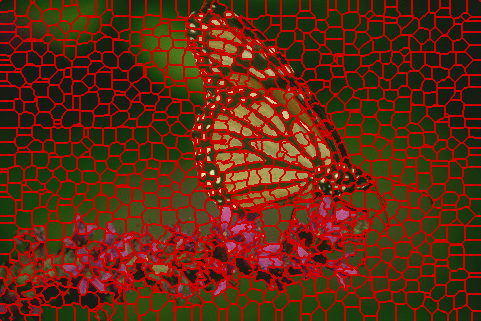
\includegraphics[width=9cm]{figuras/example-superpixel-segmentation}}
		}{
			\Fonte{\cite{SuperPixelBenchmark2017}}
		}
\end{figure}



Seguindo essa perspectiva, ao utilizar um algoritmo de extração de
\textit{features} de imagens sobre o superpixel, tem-se que o vértice
do grafo é neste momento um vetor de características. O sistema de
competição proposto no artigo \textit{Network Unfolding Map By
Vertex-Edge Dynamics Modeling} pode otimizar o pertencimento de
classes (segmentos, nesse caso) baseado na topologia de sua vizinhança
e na relação aos vértices conectados. A métrica de similaridade
(por exemplo, distância euclidiana, cosseno, etc.) pode ser
ajustada de acordo com o problema.

Ao considerar o problema como semi-supervisionado, a pista de ter
alguns dos superpixels anotados adicionaria um \textit{bias}
parametrizado pelo conhecimento do especialista em uso da ferramenta,
como um editor ou um médico. A otimização do pertencimento das classes
então seria acionada pela dinâmica coletiva selecionada em questão,
que, por acaso, poderia ser o algoritmo \gls{LCU} mencionado anteriormente.

Por outro lado, ainda há muitas melhorias a serem feitas nessas técnicas, como,
por exemplo: analisar as condições de convergência do algoritmo. Isso
pode ser um dos resultados deste trabalho, demandando uma análise
matemática com auxílio de experimentos.

É importante mencionar que já foi demonstrado em outras situações,
como em~\cite{JarbasComplexNetworks2020}, que o uso de redes complexas
em fusão com redes neurais aleatórias pode gerar um discriminante de
textura da imagem de alta relevância como extrator de
características. Neste caso, é possível se apoiar nesse resultado como
uma evidência de que a investigação de novas técnicas considerando a
topologia da imagem através de redes complexas é uma oportunidade de
pesquisa.


\section{Aplicação de Agrupamento Semissupervisionado para Segmentação
  de Imagens Coloridas}\label{sec:franciscolira2018}

Neste trabalho o autor~\cite{franciscolira2018}, na sua tese de
graduação, propõe variações de um algoritmo de segmentação de imagem
semi-supervisionado combinando algoritmos de agrupamento, como
\textit{Fuzzy C-Means}, Algoritmo de Pedrycs, Algoritmo
Semi-supervisionado Padrão (sSSC) e Algoritmo Semi-supversionado
Regularizado por Entropia (ESSC).


% LocalWords:  transdutivo superpixel

	\chapter{Metodologia}\label{cap:metodologia}


Este projeto de trabalho de conclusão de concurso foi dividido em quatro fases:
Pesquisa, Desenvolvimento, Testes e Monografia.

Durante a pesquisa científica, os artigos referenciados foram explorados com
maior atenção, ao buscar entender os detalhes que implicam
na criação da técnica proposta. Em especial, dois artigos terão maior
atenção inicialmente: \textit{Network Unfolding Map By Vertex-Edge
  Dynamics Modeling}~\cite{VerriNetworkUnfoldingMap2018} e
\textit{Image Segmentation Methods Based on Superpixel Techniques A
  Survey}~\cite{SuperpixelSurvey2020}. O primeiro contém a definição
da técnica LCU, uma dinâmica coletiva sobre redes complexas, o
componente de aprendizagem principal do algoritmo; o segundo será
usado como uma pré-segmentação inicial antes de partir pra construção
da rede complexa. Na Figura~\ref{fig:fluxograma-algoritmo} é demonstrada uma
visão macro do algoritmo.

\begin{figure}[!h]
        \captionsetup{width=8cm}
		\Caption{\label{fig:fluxograma-algoritmo}
          Algoritmo de segmentação semi-supervisionada de imagens}
		\centering
		\UFCfig{}{
			\fbox{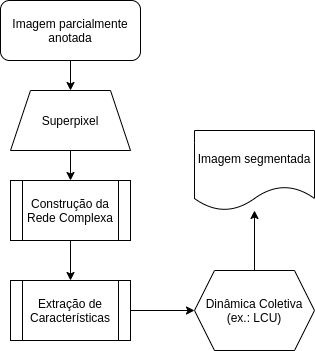
\includegraphics[width=8cm]{figuras/algorithm}}
		}{
			\Fonte{Autoral}
		}
\end{figure}


O desenvolvimento foi concentrado na integração das técnicas
mencionadas acima como uma nova técnica de segmentação de imagens
semi-supervisionada, portanto, estes detalhes são explorados na seção
de resultados sobre as etapas necessárias pra construção e aplicação
do novo algoritmo de segmentação. Por exemplo, a construção da rede
complexa assumirá que cada superpixel será um vértice do grafo com
seus vizinhos baseado na topologia da imagem, a etapa de extração de
características ocorrerá em cada superpixel e a dinâmica coletiva
considerará a anotação parcial da imagem. No fim do algoritmo, os
segmentos da imagem serão subgrafos dessa rede complexa.

Adicionalmente, a implementação do algoritmo nesse trabalho foi
construída de maneira \textit{Open Source} como uma ferramenta de
simulação de segmentação, usando a biblioteca \gls{OpenCV} para que possa
ser testado o algoritmo de segmentação de imagens recebendo pontos
aleatórios de marcação do usuário. Isto simula o caso de um
especialista analisando uma imagem médica, por exemplo.

Na fase de testes, a avaliação dos resultados foi considerado os
principais \textit{datasets} conhecidos para segmentação de imagens,
como o \textit{The Berkeley Segmentation Dataset and Benchmark}
~\cite{MartinFTM01}. É também realizado variações no algoritmo, como
diferentes abordagens para extração de características e variação de
parâmetros na dinâmica coletiva.

Na fase de monografia foram consolidados todos os resultados em um
trabalho acadêmico nas normas da \gls{ABNT}.

	\chapter{RESULTADOS}\label{chap:resultados}

Uma implementação do algoritmo EGSIS foi realizada como um projeto de
código-aberto e está disponível na plataforma
github\footnotemark. Nessa seção de resultados, avalia-se o
comportamento do método com variações no número de superpixels e
método de extração de características. Como referência para comparação
dos resultados, considera-se os métodos avaliados
em~\cite{wang2023review} no \textit{dataset} GrabCut.

\footnotetext{Disponível em \url{https://github.com/ryukinix/egsis/releases/tag/0.1.0}}

Uma avaliação qualitativa é demonstrada ao realizar a segmentação do
método e disponibilizar a máscara de segmentação gerada para algumas
imagens. Além disso, em formato de tabelas, é disponibilizada a
avaliação quantitativa baseada nas métricas descritas na
seção~\ref{sec:metricas-avaliacao}.

Por fim, foi desenvolvida uma ferramenta simples de anotação para
exploração dos resultados integrada ao software
JupyterLab\footnotemark, que é usada também para avaliação qualitativa
e visualização do impacto da anotação parcial inicial no resultado
final.

\footnotetext{Software web para desenvolvimento interativo e análise de dados, disponível em \url{https://jupyter.org}}

\section{Experimentos com a variação da quantidade de superpixels}\label{sec:variacao-superpixels}

Durante a execução dos experimentos, e avaliação dos resultados, foi
observado que o número de superpixels afeta diretamente a qualidade da
segmentação gerada. Entre esses experimentos, foram realizadas 8
execuções com variações na técnica de extração de características
usada e no número de superpixels, sendo o número de superpixels
avaliados para 50, 100, 150 e 200.

\begin{table}[!h]
    \centering
    \Caption{\label{tab:variacao-superpixels} Resultados dos
experimentos ao variar o número de superpixels e o método de extração
de características. Em negrito os melhores resultados.}
  \begin{tabular}{lcccc}
    \toprule
    \textbf{Método}                  & \textbf{Recall} & \textbf{Precision} & \textbf{F1}     & \textbf{IoU}    \\
    \midrule \midrule
    $\gls{EGSIS}(s=50, f=gabor)$     & 0.7882          & 0.9225             & 0.8414          & 0.7412          \\
    $\gls{EGSIS}(s=100, f=gabor)$    & 0.8592          & 0.9505             & 0.8992          & 0.8232          \\
    $\gls{EGSIS}(s=150, f=gabor)$    & 0.8691          & 0.9550             & 0.9066          & 0.8354          \\
    $\gls{EGSIS}(s=200, f=gabor)$    & 0.8799          & \textbf{0.9620}    & 0.9167          & 0.8511          \\
    $\gls{EGSIS}(s=50, f=comatrix)$  & 0.7882          & 0.9225             & 0.8414          & 0.7412          \\
    $\gls{EGSIS}(s=100, f=comatrix)$ & 0.8617          & 0.9510             & 0.9010          & 0.8259          \\
    $\gls{EGSIS}(s=150, f=comatrix)$ & 0.8777          & 0.9552             & 0.9125          & 0.8441          \\
    $\gls{EGSIS}(s=200, f=comatrix)$ & \textbf{0.8877} & 0.9611             & \textbf{0.9212} & \textbf{0.8578} \\
    \bottomrule
  \end{tabular}
  \Fonte{\fonteautor}
\end{table}

Ao analisar a tabela~\ref{tab:variacao-superpixels}, é possível
perceber que o aumento de superpixels impacta positivamente na
qualidade da segmentação independente do método de extração de
características. A respeito do método de extração de características,
os resultados de ambos os métodos são próximos. Por outro lado, com
exceção da métrica de precisão, os melhores resultados vieram do
modelo com 200 superpixels e extração de características via matriz de
co-ocorrências.


\section{Avaliação qualitativa}

Nesta avaliação qualitativa, é comparada visualmente a qualidade
de segmentação do método \gls{EGSIS} com os melhores parâmetros
encontrados na seção anterior, isto é, número de superpixels definido
para 200 e método de extração de características via matriz de
co-ocorrências.

Como referência, o artigo~\cite{wang2023review} contém execuções
comparativas de vários métodos na base de dados GrabCut. Neste artigo,
é selecionada uma comparação com 16 imagens, nas quais 7 diferentes
métodos de segmentação interativa foram usados.

\begin{figure}[h!]
        \captionsetup{width=16cm}
		\Caption{\label{fig:grabcut-comparacao}
          Comparação entre diferentes métodos de segmentação interativa no dataset GrabCut.
        }
		\centering
		\UFCfig{}{\fbox{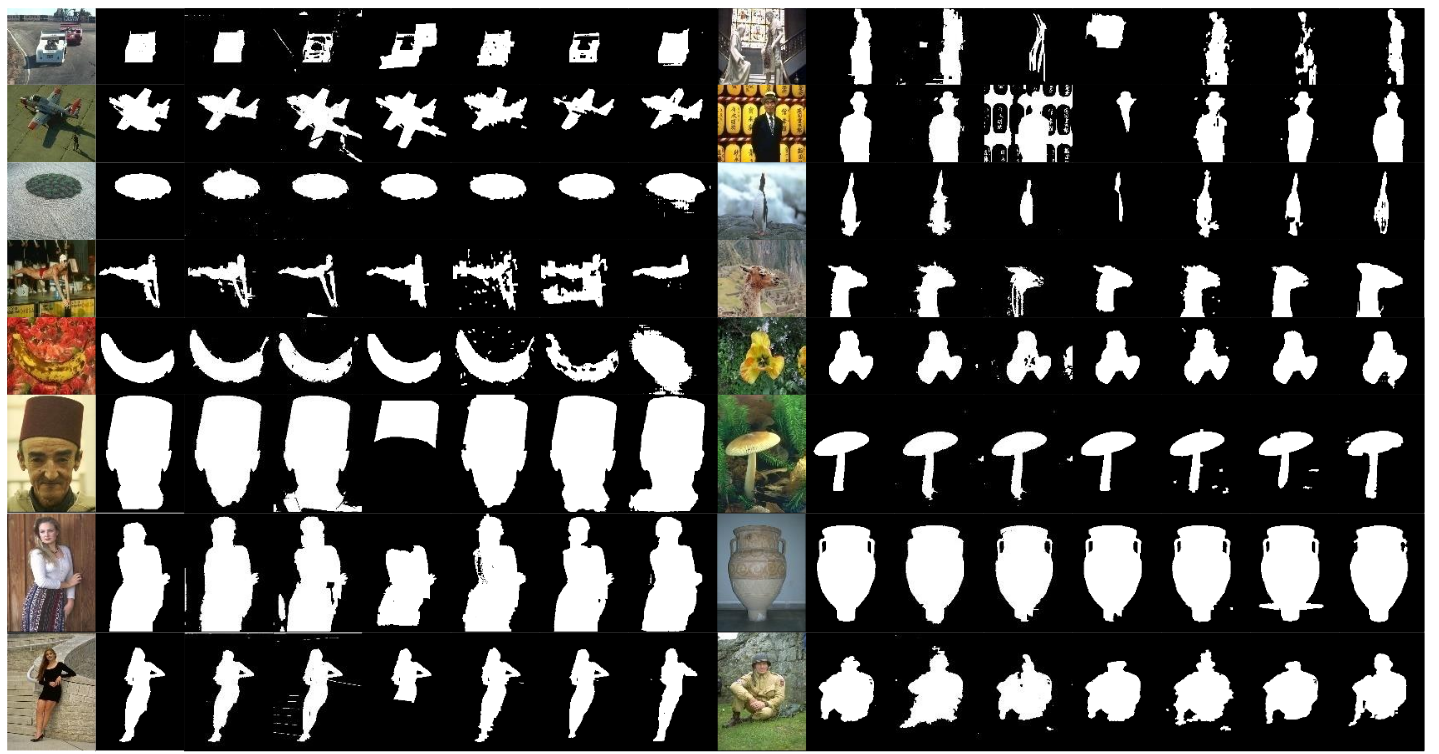
\includegraphics[width=16cm]{figuras/grabcut-comparacao}}}{\Fonte{\cite{wang2023review}}}
\end{figure}
\FloatBarrier{}

Na Figura~\ref{fig:grabcut-comparacao}, há em cada linha duas
imagens a serem segmentadas. Entre as máscaras de segmentação em escala
de cinza, há as segmentações dos métodos de segmentação
interativa. O nome desses 7 métodos, em ordem, são: GrabCut,
LazySnapping, OneCut, Saliency Cut, Iterated Graph Cuts, DenseCut e
Deep GrabCut.

Nesse aspecto, para comparação com o modelo proposto \gls{EGSIS}, para
as mesmas imagens do dataset GrabCut, são obtidas as seguintes máscaras
de segmentação na Figura~\ref{fig:egsis-qualitativa}.

\begin{figure}[h!]
        \captionsetup{width=11.5cm}
		\Caption{\label{fig:egsis-qualitativa}
          Execução de segmentação interativa com EGSIS, a primeira
segmentação é a do modelo e a última é a segmentação real.
        }
		\centering
		\UFCfig{}{\fbox{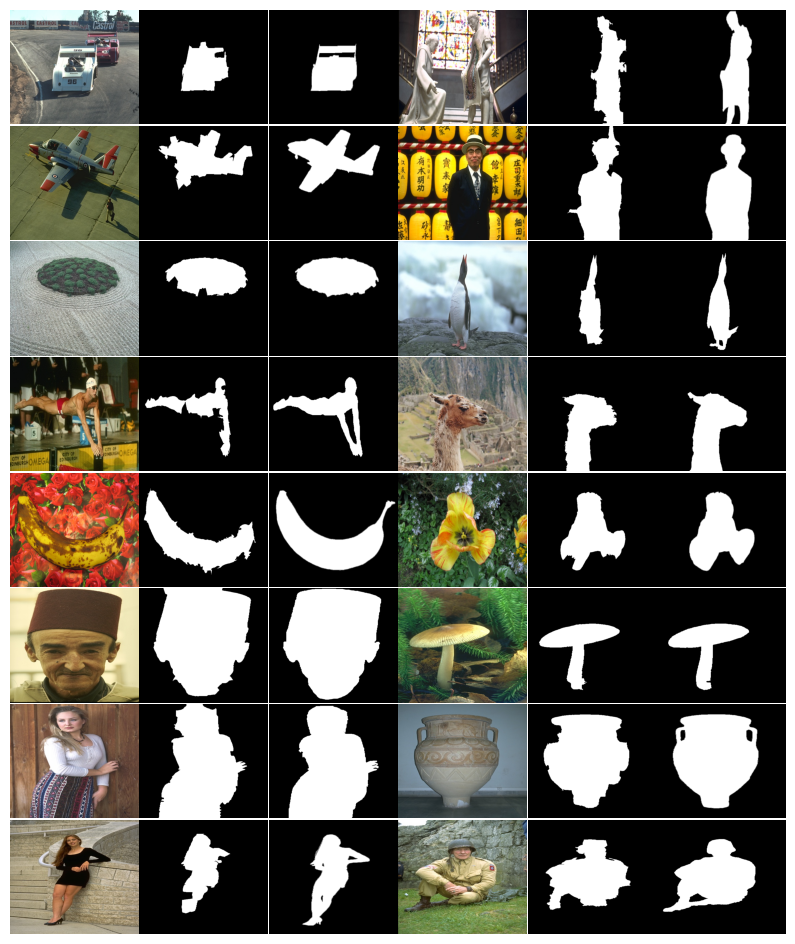
\includegraphics[width=11.5cm]{figuras/egsis-qualitativa}}}{\Fonte{\fonteautor}}
\end{figure}
\FloatBarrier{}



Como pode ser visto, os resultados do \gls{EGSIS} são de qualidade
equiparável aos métodos de referência em~\citeonline{wang2023review}, embora em
algumas imagens haja mais erros e outras obtenham maior êxito. Para
quantificar esse resultado, na próxima
seção~\ref{sec:comparacao-estado-da-arte} é realizada uma avaliação
quantitativa comparando esses métodos e o método proposto \gls{EGSIS}.


\section{Comparação quantitativa com o estado-da-arte da segmentação interativa}\label{sec:comparacao-estado-da-arte}

Nesta seção, é proposta uma avaliação de como o modelo \gls{EGSIS} se
compara ao estado-da-arte no problema de segmentação interativa.

No artigo~\citeonline{wang2023review}, é observado um extenso estudo de
revisão sobre os métodos de segmentação interativa baseados em grafos,
tendo como base o algoritmo GrabCut e outros algoritmos que evoluíram
nessa área de segmentação interativa de imagens. Os autores avaliam
essas técnicas na base de dados GrabCut~\cite{rother2004grabcut}
utilizando as mesmas métricas que foram selecionadas na metodologia de
avaliação deste trabalho, com exceção do tempo de execução, que, por
conta de diferentes tecnologias usadas para implementação das
técnicas, não foi possível usar para fazer uma avaliação justa, por
isso será deixada como um potencial trabalho futuro.

Esse mesmo artigo também avalia as várias técnicas em outro
\textit{dataset}, mas em virtude de a rotulação inicial usada não ter
sido publicada, não foi possível replicar os experimentos para o
modelo \gls{EGSIS} nas mesmas condições. Por esse motivo, a avaliação
de resultados será limitada a base de dados GrabCut.

A seguir, é possível visualizar tabelas de comparação com os
algoritmos apresentados em~\citeonline{wang2023review}: GrabCut,
LazySnapping, OneCut, Saliency Cut, Iterated Graph Cuts, DenseCut e
Deep GrabCut, todos algoritmos de segmentação interativa baseado em grafos.


\begin{table}[!h]
    \centering
    \Caption{\label{tab:resultados-estado-da-arte} Resultados
      comparativos entre o método EGSIS e métodos estado-da-arte para
      segmentação interativa baseado em grafos. Em negrito os melhores
      resultados, em vermelho os piores.}
  \begin{tabular}{lcccc}
    \toprule
    \textbf{Método}                    & \textbf{Recall} & \textbf{Precision} & \textbf{F1}     & \textbf{IoU}    \\
    \midrule \midrule
    GrabCut                            & 0.9668          & 0.9213             & \textbf{0.9407} & \textbf{0.8927} \\
    LazySnapping                       & \textbf{0.9681} & 0.9104             & 0.9357          & 0.8842          \\
    OneCut                             & 0.8585          & \red{0.7926}       & \red{0.7899}    & \red{0.6974}    \\
    Saliency Cuts                      & \red{0.8371}    & 0.8892             & 0.8255          & 0.7458          \\
    Iterated Graph Cuts\footnotemark{} & 0.9614          & 0.8878             & 0.9212          & 0.8597          \\
    DenseCut                           & 0.8427          & 0.9418             & 0.8561          & 0.7927          \\
    Deep GrabCut                       & 0.8854          & 0.8774             & 0.8701          & 0.7849          \\
    $\gls{EGSIS}(s=200, f=gabor)$      & 0.8799          & \textbf{0.9620}    & 0.9167          & 0.8511          \\
    $\gls{EGSIS}(s=200, f=comatrix)$   & 0.8877          & 0.9611             & 0.9212          & 0.8578          \\
    \bottomrule
  \end{tabular}
  \Fonte{Baseado nos resultados encontrados no artigo~\cite{wang2023review}}
\end{table}
\FloatBarrier{}

\footnotetext{Não há um nome formal pra esse método~\cite{an2013iterated}, por ora ele será chamado assim}

Na tabela~\ref{tab:resultados-estado-da-arte}, é possível
observar que o método $\gls{EGSIS}(s=200, f=gabor)$ atinge o maior
valor médio de precisão entre todos os métodos comparados, com um
valor de 0.9620. Seguindo o método EGSIS, o segundo colocado na
métrica de precisão foi o método DenseCut, com um valor de precisão de
0.9418, que é próximo, mas ainda significativamente menor. É
importante ressaltar que uma alta precisão implica uma baixa
incidência de pixels falsos-positivos.

Em nenhuma das métricas apresentadas na comparação o EGSIS se
classifica como o pior método. No entanto, observa-se um valor menor
de \textit{recall} em comparação à precisão, o que impacta diretamente
no valor das métricas \textit{F1} e IoU. Neste cenário, conclui-se que
o modelo EGSIS tem uma taxa maior de falsos-negativos do que de
falsos-positivos.

Embora seja necessária uma investigação mais aprofundada para
determinar a causa dessa maior taxa de falsos-negativos, é importante
notar que o conjunto de dados GrabCut possui um desequilíbrio na
quantidade de pixels entre as classes, sendo o plano de fundo a classe
dominante. No algoritmo \gls{LCU}, um dos fatores importantes para
classificar um vértice que representa um superpixel é a extração de
características que através de uma função de similaridade calcula o
peso das arestas da rede complexa. No entanto, esse é apenas um dos
fatores do sistema dinâmico, pois também há a geração de partículas e
a transição entre os vértices. Geralmente, o objeto é cercado pelo
plano de fundo. Isso pode levar a uma situação onde a rede complexa
maior, localizada fora do objeto, gera partículas da classe do plano
de fundo em quantidade suficiente para dominar os vértices na região
do objeto. Esse comportamento implicaria um aumento na incidência de
falsos-negativos.

Se isso for confirmado, uma possível contramedida seria modificar o
sistema dinâmico para dar maior peso às similaridades entre
superpixels, de tal maneira que haja um aumento da probabilidade
de sobrevivência das partículas entre superpixels de mesma
classe. Além disso, seria útil explorar novas técnicas de extração de
características que gerem valores de similaridade mais
discriminantes. Essas ideias serão discutidas com mais detalhes na
próxima seção deste trabalho.

	\chapter{Conclusões e Trabalhos Futuros}
\label{chap:conclusoes-e-trabalhos-futuros}

Em desenvolvimento...

%\label{sec:contribuicoes-do-trabalho}



%\label{sec:limitacoes}


	%Elementos pós-textuais
	\bibliography{3-pos-textuais/referencias}
    %\imprimirglossario
	% \imprimirapendices
	% 	% Adicione aqui os apendices do seu trabalho
	% 	\apendice{Exemplo de apêndice}
\label{ap:A}

Um apêndice é um documento elaborado pelo autor, diferentemente do anexo. Geralmente, se coloca como apêndice, questionários, códigos de programação, tabelas que tomariam muito espaço no meio do trabalho. Artigos, resumos ou qualquer publicação relacionada ao trabalho podem ser utilizados como apêndice.
	% 	\apendice{Questionário utilizado para...}
\label{ap:B}

\begin{questao}
	\item Esta é a primeira questão com alguns itens:
		\begin{enumerate}
			\item Este é o primeiro item
			\item Segundo item
		\end{enumerate}
	\item Esta é a segunda questão:
		\begin{enumerate}
			\item Este é o primeiro item
			\item Segundo item
		\end{enumerate}
	\item Lorem ipsum dolor sit amet, consectetur adipiscing elit. Nunc dictum sed tortor nec viverra. consectetur adipiscing elit. Nunc dictum sed tortor nec viverra.
		\begin{enumerate}
			\item consectetur
			\item adipiscing
			\item Nunc
			\item dictum
		\end{enumerate}
\end{questao}

	% 	\apendice{Códigos-fontes utilizados para...}
\label{ap:C}

\lstinputlisting[language=C++,caption={Hello World em C++}]{figuras/main.cpp}


\begin{lstlisting}[language=Java,caption={Hello World em Java}]
public class HelloWorld {
	public static void main(String[] args) {
		System.out.println("Hello World!");
	}
}
\end{lstlisting}


	% 	\apendice{\textit{IEEE CEFC 2016}}
\label{ap:D}

\textit{Digest} submetido ao \textit{The 17th Biennial Conference on Eletromagnetic Field Computation, Miami FL - NOV 13-16, 2016, USA}.

%Código fonte para inserir um arquivo em PDF
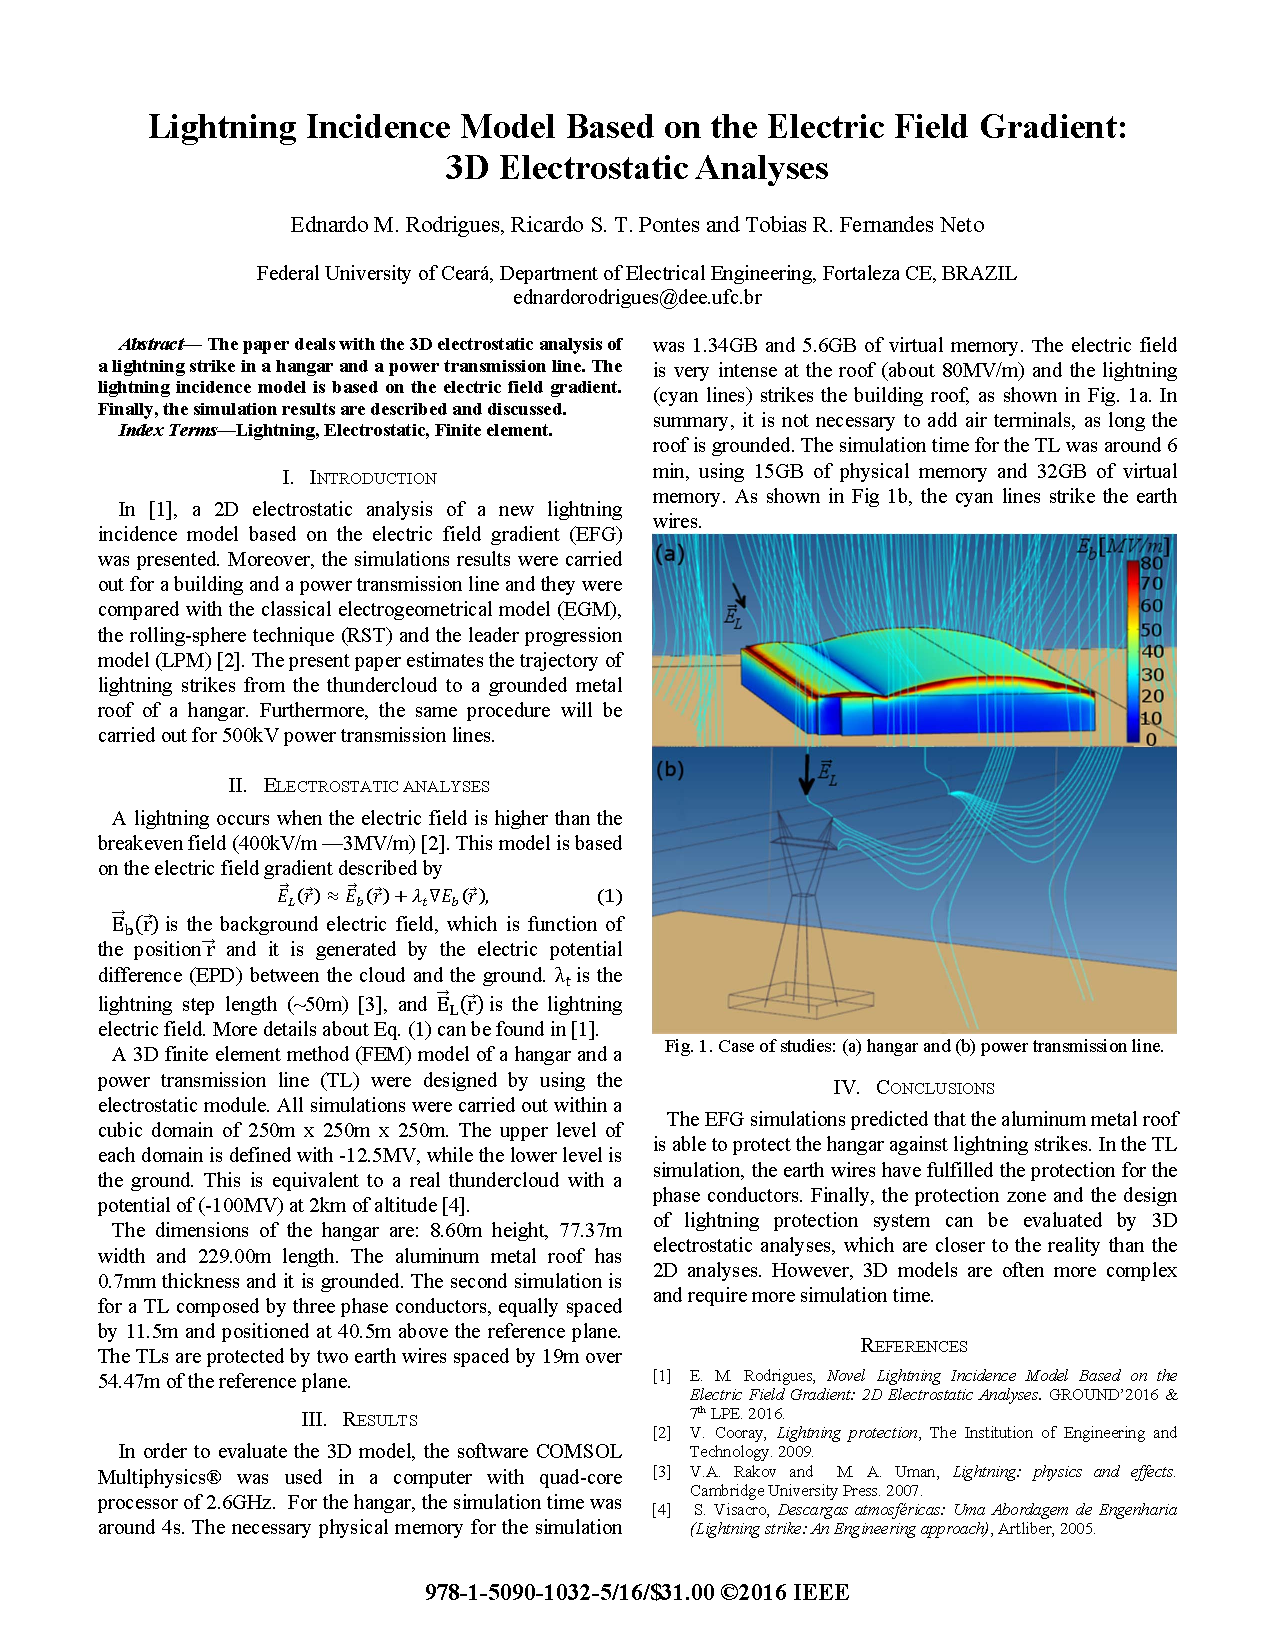
\includepdf[pages={-}]{3-pos-textuais/apendices/PID4416093.pdf}
	% \imprimiranexos
	% 	% Adicione aqui os anexos do seu trabalho
	% 	\anexo{Exemplo de um anexo}
\label{an:ex_anexo_a}

Um anexo é um documento que não foi elaborado pelo autor, ou seja, o autor apenas anexa. Anexos podem ser tabelas, mapas, diagramas, \textit{datasheets}, manuais e etc. 




	% 	\anexo{Exemplo de um anexo em PDF}
\label{an:ex_anexo_b}

O autor pode anexar um \gls{PDF}, traduzido como formato portátil de documento. Veja o código fonte utilizado para anexar o arquivo ``Sikasil.pdf'' que foi colocado dentro da pasta ``anexos'' que por sua vez está dentro da pasta ``elementos-pos-textuais''. Tenha muita atenção na hora de especificar o local do arquivo. Recomenda-se não utilizar caracteres especiais para nomear pastas e, principalmente, arquivos. 

Pode-se fazer uma descrição sucinta do arquivo anexado.

%Comando para incluir um arquivo em PDF:
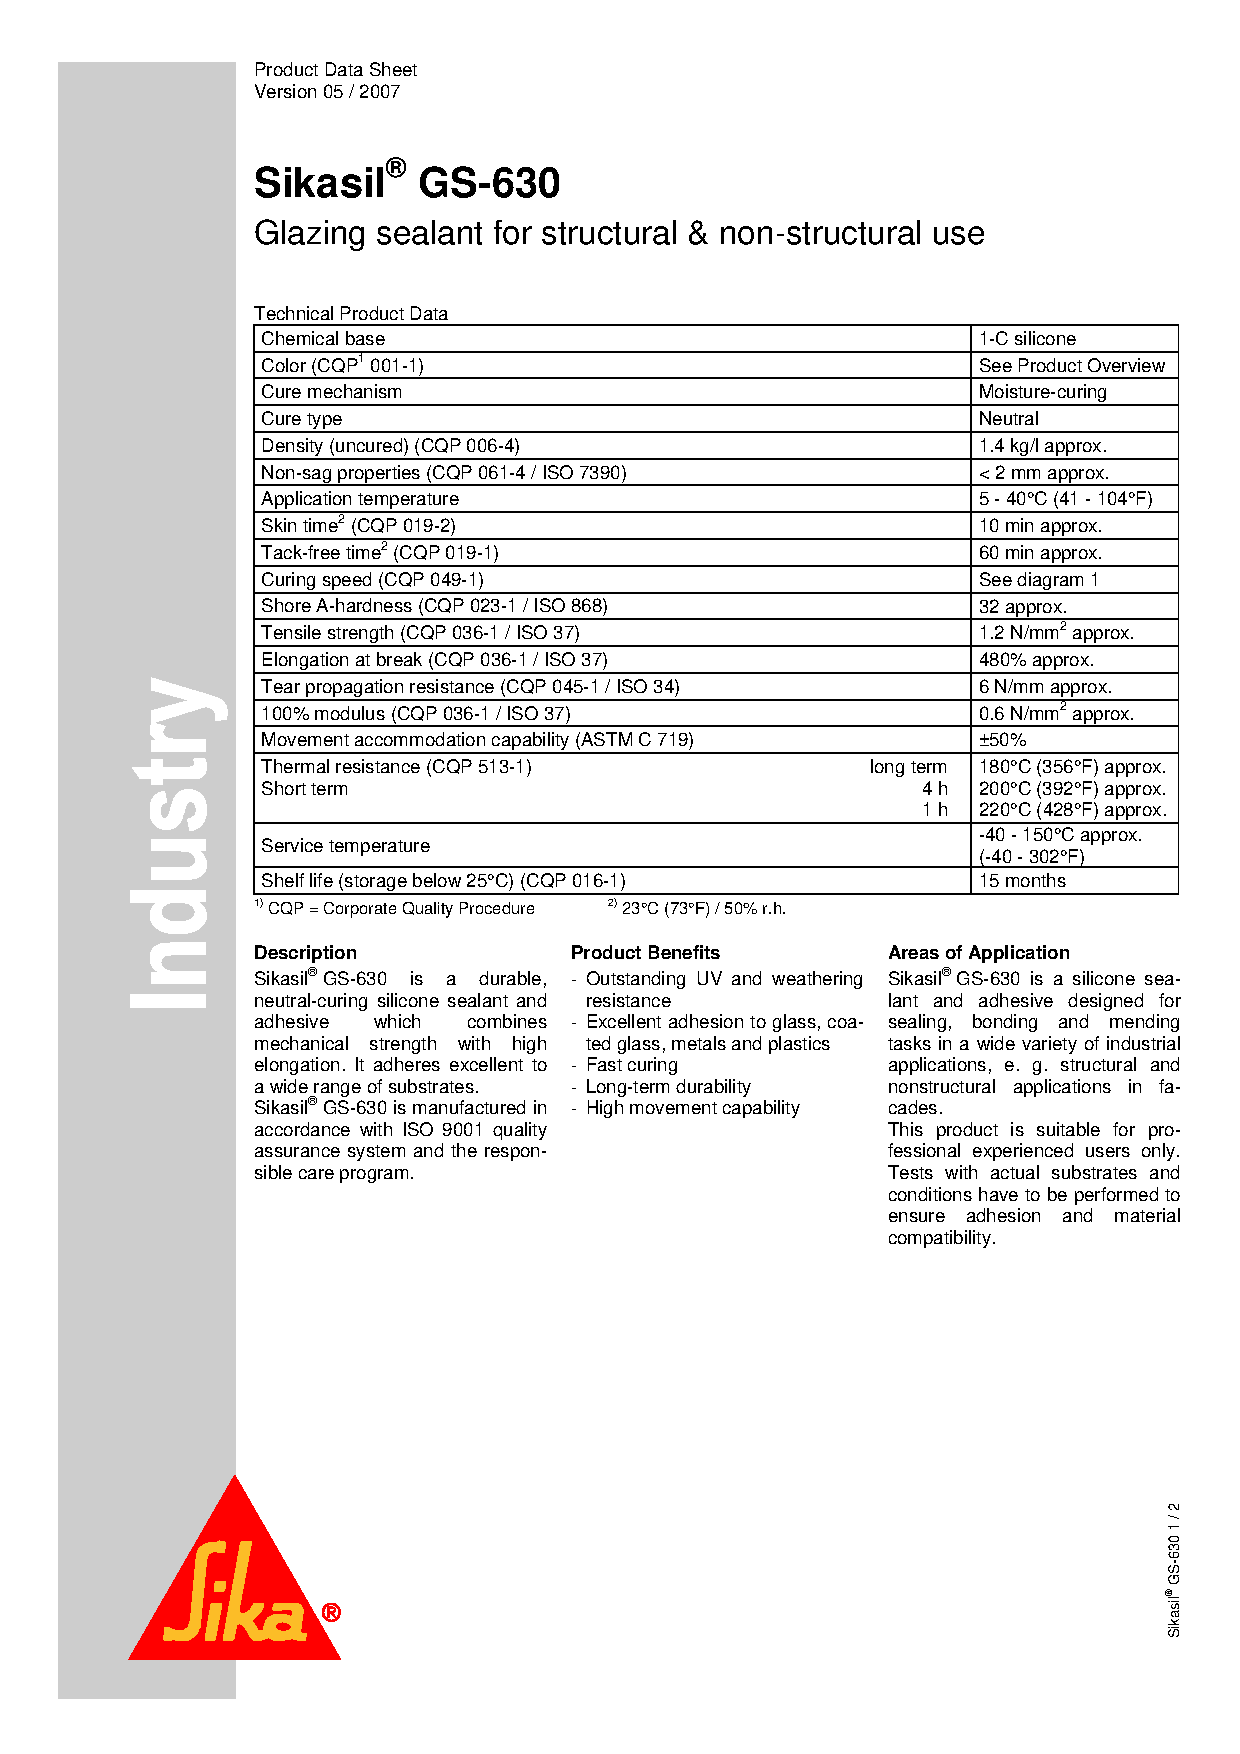
\includepdf[pages={-}]{3-pos-textuais/anexos/Sikasil.pdf}


	% \imprimirindice

\end{document}

% chktex-file 1
